\documentclass{article}

% 导入宏包
\usepackage{fancyhdr}
\usepackage{ctex}
\usepackage{listings}
\usepackage{graphicx}
\usepackage[a4paper, body={18cm,22cm}]{geometry}
\usepackage{amsmath,amssymb,amstext,wasysym,enumerate,graphicx}
\usepackage{float,abstract,booktabs,indentfirst,amsmath}
\usepackage{array}
\usepackage{multirow}
\usepackage{url}
\usepackage{diagbox}
\usepackage{enumitem}
\usepackage{xcolor}
\usepackage{makecell}
\usepackage{tikz}
\usetikzlibrary{positioning, arrows.meta}

% 设置段落
\renewcommand\arraystretch{1.4}
\setlength{\parindent}{2em}
\setCJKmonofont{黑体}

% 配置代码显示
\lstset{
	xleftmargin = 3em,
	xrightmargin = 3em,
	aboveskip = 1em,
	backgroundcolor = \color{white},
	basicstyle = \small\ttfamily,
	rulesepcolor = \color{gray},
	breaklines = true,
	numbers = left,
	numberstyle = \small,
	numbersep = -14pt,
	keywordstyle = \color{purple}\bfseries,
	commentstyle = \color{green!60!black}, % 修改注释颜色
	stringstyle = \color{red!60!green!90!blue!90},
	morekeywords = {ASSERT, int64_t, uint32_t},
	moreemph = {ASSERT, NULL},
	emphstyle = \color{red}\bfseries,
	moreemph = [2]{int64\_t, uint32\_t, tid\_t, uint8\_t, int16\_t, uint16\_t, int32\_t, size\_t, bool},
	emphstyle = [2]\color{purple}\bfseries,
	frame = shadowbox,
	showspaces = false,
	columns = fixed
	morecomment = [l][\color{green!60!black}]{+}, % 设置以+开头的代码行为绿色
}

%--------------------页眉--------------------%

\pagestyle{fancy}
\fancyhead[L]{}
\fancyhead[R]{}
\fancyhead[C]{华东师范大学软件工程学院实验报告}
\fancyfoot[C]{-\thepage-}
\renewcommand{\headrulewidth}{1.5pt}

%--------------------标题--------------------%

\begin{document}
	\begin{center}
		{\Large{\textbf{\heiti 华东师范大学软件工程学院实验报告}}}
		\begin{table}[htb]
			\flushleft
			\begin{tabular}{p{0.4\linewidth}p{0.27\linewidth}p{0.28\linewidth}}\\
				\textbf{实验课程}:计算机网络实践  & \textbf{年级}:2023级       & \textbf{实验成绩}:  \\
				\textbf{实验名称}:IPV4 & \textbf{姓名}:顾翌炜         &                 \\
				\textbf{实验编号}:Lab-3     & \textbf{学号}:10235101527 & \textbf{实验日期}:2024/12/06  \\
				\textbf{指导教师}:王廷     & \textbf{组号}:01            & \textbf{实验时间}:2024/12/06  \\ 
			\end{tabular}
		\end{table}
	\end{center}
	\rule{\textwidth}{2pt}
	
	%--------------------正文--------------------%
	\section{实验目的}
	
	\begin{enumerate}[noitemsep, label={{\arabic*})}]
		\item 学会通过 \texttt{Wireshark} 分析 \texttt{IP} 协议
		\item 了解 \texttt{IP} 数据报的组成
		\item 了解 \texttt{IP} 各部分的含义
	\end{enumerate}
	
	\section{实验内容和实验步骤}
	
	\subsection{实验内容}
	
	\subsubsection{数据捕获}
	\begin{enumerate}
		\item 启动 Wireshark 应用程序。
		\item 通过菜单栏选择“捕获”→“选项”进行设置。
		\item 选择已连接的以太网接口。
		\item 设置捕获过滤器为 \texttt{tcp port 80} 以捕获通过 HTTP 端口的数据包。
		\item 在命令行界面使用 \texttt{wget} 命令向 \texttt{http://www.baidu.com} 发送 HTTP 请求。
		\item 打开 Wireshark 的捕获窗口,并在适当时候停止捕获过程。
	\end{enumerate}
	
	\subsubsection{分析 IPv4 包结构}
	根据对 IP 报文的理解,绘制出 IP 报文的结构图。在图中明确标注 IP 报头字段的位置及其大小(以字节为单位)。
	
	\subsubsection{数据包分析}
	对捕获到的 IP 数据包进行详细分析,关注以下字段的含义:
	\begin{enumerate}
		\item \textbf{版本号 (Version)}: 占用 4 位。用于指示当前使用的 IP 协议版本,常见值为 0100(代表 IPv4),0110(代表 IPv6)。
		\item \textbf{首部长度 (Header Length)}: 占用 4 位。用于说明 IP 报头的总长度,考虑到 IP 报头中存在可变长度的选项字段。
		\item \textbf{区分服务 (Differentiated Services)}: 占用 8 位。用于为不同的 IP 数据包指定不同的服务质量。
		\item \textbf{总长度 (Total Length)}: 占用 16 位。表示 IP 包的总大小(包括头部和数据),单位为字节,最大值为 65535 字节。有效载荷的大小计算公式为:IP 包总长度 (Total Length) 减去 IP 报头长度 (Header Length)。
		\item \textbf{标识 (Identifier)}: 长度 16 位。与 Flags 和 Fragment Offset 字段联合使用,用于对较大的数据报进行分段操作。所有拆分的分段将被标记为相同的值,以便于目的端设备能够识别各个分段属于同一数据报的一部分。
		\item \textbf{标志 (Flags)}: 长度 3 位,第一位不使用。第二位是 DF (Don't Fragment) 位,当 DF=1 时,表明路由器不能对该数据报进行分段。第三位是 MF (More Fragments) 位,MF=1 表示后续还有更多的分片,MF=0 则表示当前分片是数据报的最后一个。
		\item \textbf{片偏移 (Fragment Offset)}: 长度 13 位,以 8 个字节为偏移单位。此字段指示接收端该分片在原始数据报中的相对位置,从而确定分片在数据报数据部分的起始位置,便于重组还原原始 IP 包。
		\item \textbf{生存时间 (TTL)}: 长度 8 位,以跳数为单位。此字段表示数据报在网络中传输过程中能经过的最大跳数。每经过一个三层设备(如路由器),TTL 值减 1。当 TTL 降至 0 时,数据报将被丢弃,防止因路由环路导致数据报在网络中无限循环。
		\item \textbf{协议 (Protocol)}: 长度 8 位,用于标识上层协议。
		\item \textbf{首部校验和 (Header Checksum)}: 长度 16 位,用于验证 IP 头部的正确性,但不包括数据部分。
	\end{enumerate}
	
	\subsubsection{回答问题}
	
	By looking at the IP packets in your trace, answer these questions:
	
	\begin{enumerate}
		\item What are the IP addresses of your computer and the remote server?
		\item Does the Total Length field include the IP header plus IP payload, or just the IP payload?
		\item How does the value of the Identification field change or stay the same for different packets? For instance, does it hold the same value for all packets in a TCP connection or does it differ for each packet? Is it the same in both directions? Can you see any pattern if the value does change?
		\item What is the initial value of the TTL field for packets sent from your computer? Is it the maximum possible value, or some lower value?
		\item How can you tell from looking at a packet that it has not been fragmented? Most often IP packets in normal operation are not fragmented. But the receiver must have a way to be sure. Hint: you may need to read your text to confirm a guess.
		\item What is the length of the IP Header and how is this encoded in the header length field? Hint: notice that only 4 bits are used for this field, as the version takes up the other 4 bits of the byte. You may guess and check your text.
	\end{enumerate}
	
	Hand in your drawing of an IP packet and the answers to the questions above.
	
	\subsubsection{Internet Path}
	
	在命令行下使用 \texttt{tracert} 命令,查看到达 \url{www.baidu.com} 的路由路径。根据输出画出网络路径。
	
	\subsubsection{计算 Checksum}
	
	IP报头的校验和可以用来验证一个数据包是否正确。
	
	选择一个IP报文,计算它的 checksum。计算对IP首部检验和的算法如下:
	
	\begin{enumerate}[label=(\arabic*)] % 使用圆括号和阿拉伯数字作为标签
		\item 初始化IP数据包的校验和字段,将其值设为零。
		\item 将IP首部视为16位(即2字节)的数字序列,并对这些数字执行连续的二进制加法运算。在此过程中,必须保留从最高有效位(MSB)溢出的进位,因此应使用32位加法来确保准确性。
		\item 在加法运算中,如果产生进位,则将此进位加到结果的低16位上。在32位加法的情况下,这意味着在将高16位与低16位相加后,还需将此次加法中高16位产生的任何进位添加到低16位的总和中。
		\item 最后,将得到的总和进行位取反操作,以生成校验和。
	\end{enumerate}
	
	\subsubsection{问题讨论}
	
	We encourage you to explore IP on your own once you have completed this lab. Some ideas:
	
	\begin{enumerate}
		\item Read about and experiment with IPv6. Modern operating systems already include support for IPv6 so you may be able to capture IPv6 traffic on your network. You can also "join the IPv6 backbone" by tunneling to an IPv6 provider.
		\item Learn about tunnels, which wrap an IP packet within another IP header.
		\item Read about IP geolocation, it is the process of assigning a geographical location to an IP address using measurements or clues from its name administrative databases. Try a geolocation service.
		\item Learn about IPsec or IP security. It provides confidentiality and authentication for IP packets, and is often used as part of VPNs.
	\end{enumerate}
	
	\subsection{实验步骤}
	
	\begin{enumerate}
		\item 启动 Wireshark,在菜单栏中选择“捕获”→“选项”进行设置。选择已连接的以太网接口,设置捕获过滤器为 \texttt{tcp port 80},关闭混杂模式,并勾选 \texttt{enable network name resolution}。之后,开始捕获数据。
		\item 切换回命令行界面,使用 \texttt{wget} 命令发起 HTTP 请求。
		\begin{lstlisting}[language=bash]
        C:\User\GHOST> wget http://www.baidu.com
		\end{lstlisting}
		\item 返回到 Wireshark,停止数据捕获。
		\item 对捕获的 IP 数据报进行分析,并绘制其结构图。
		\item 对捕获的 IP 数据报进行详细数据分析,并回答相关的分析问题。
		\item 在命令行中使用 \texttt{tracert} 命令,查看到达 \url{www.baidu.com} 的路由路径。
		\begin{lstlisting}[language=bash]
        C:\User\GHOST> tracert www.baidu.com
		\end{lstlisting}
		\item 选择一个 IP 数据报,计算其校验和(checksum)。
		\item 进行问题讨论。
	\end{enumerate}
	
	\section{实验环境}
	
	\begin{itemize}[noitemsep]
		\item 操作系统:\texttt{Windows 11 家庭中文版 23H2 22631.4460}
		\item 网络适配器:\texttt{Killer(R)Wi-Fi 6E AX1675i 160MHz Wireless Network Adapter(211NGW)}
		\item \texttt{Wireshark}:\texttt{Version 4.4.1}
		\item \texttt{wget}:\texttt{GNU Wget 1.21.4 built on mingw32}
	\end{itemize}
	
	\section{实验过程与分析}
	
	\subsection{捕获数据}
	
	首先,我们启动 \texttt{Wireshark},在菜单栏选择捕获,并进行以下设置,连接已连接的以太网,捕获过滤器为 \texttt{tcp port 80},捕获 \texttt{IP} 数据报。
	
	\clearpage
	
	\begin{figure}[H]
		\centering
		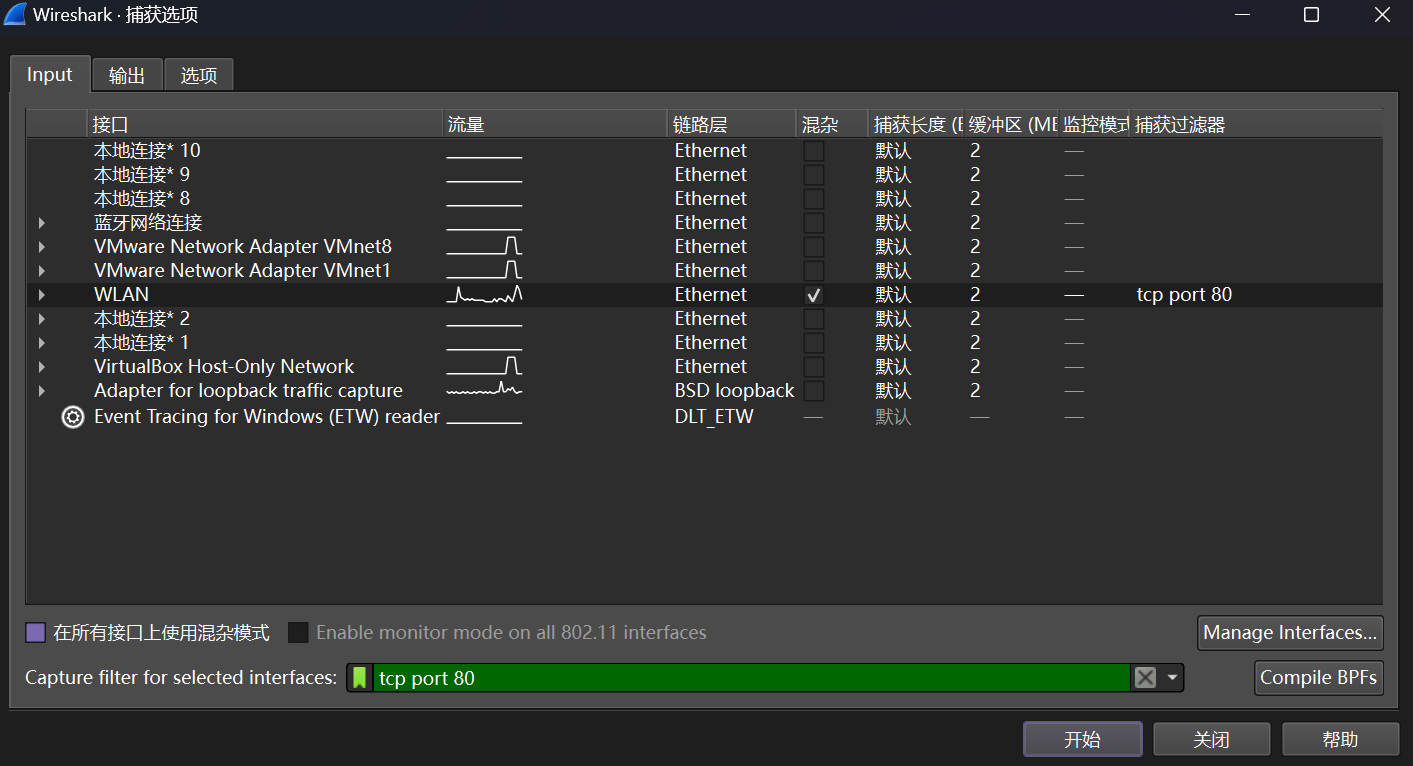
\includegraphics[width=11cm]{images/1. 设置捕获.jpg}
		\caption{设置捕获}
	\end{figure}
	
	然后在命令行使用 \texttt{wget} 指令,向 \texttt{www.baidu.com} 发送 \texttt{HTTP} 请求:
	
	\begin{figure}[H]
		\centering
		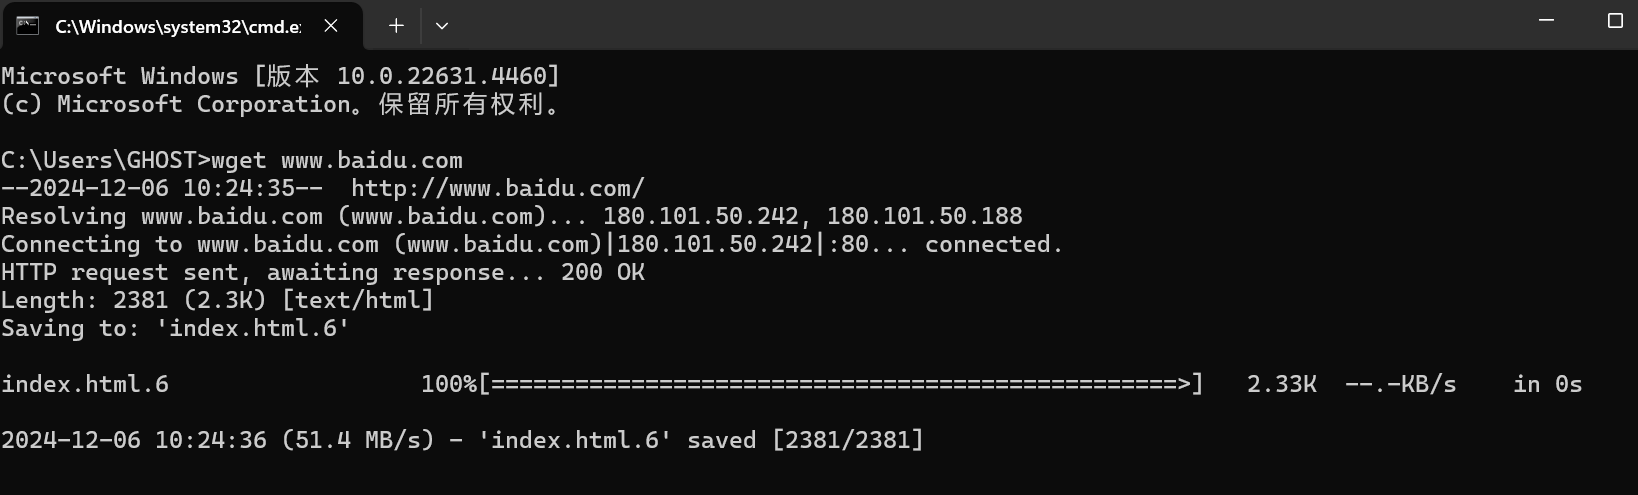
\includegraphics[width=11cm]{images/2. wget发送http请求.png}
		\caption{wget发送http请求}
	\end{figure}
	
	打开 \texttt{Wireshark} 的捕获窗口,停止捕获,得到了以下结果:
	
	\begin{figure}[H]
		\centering
		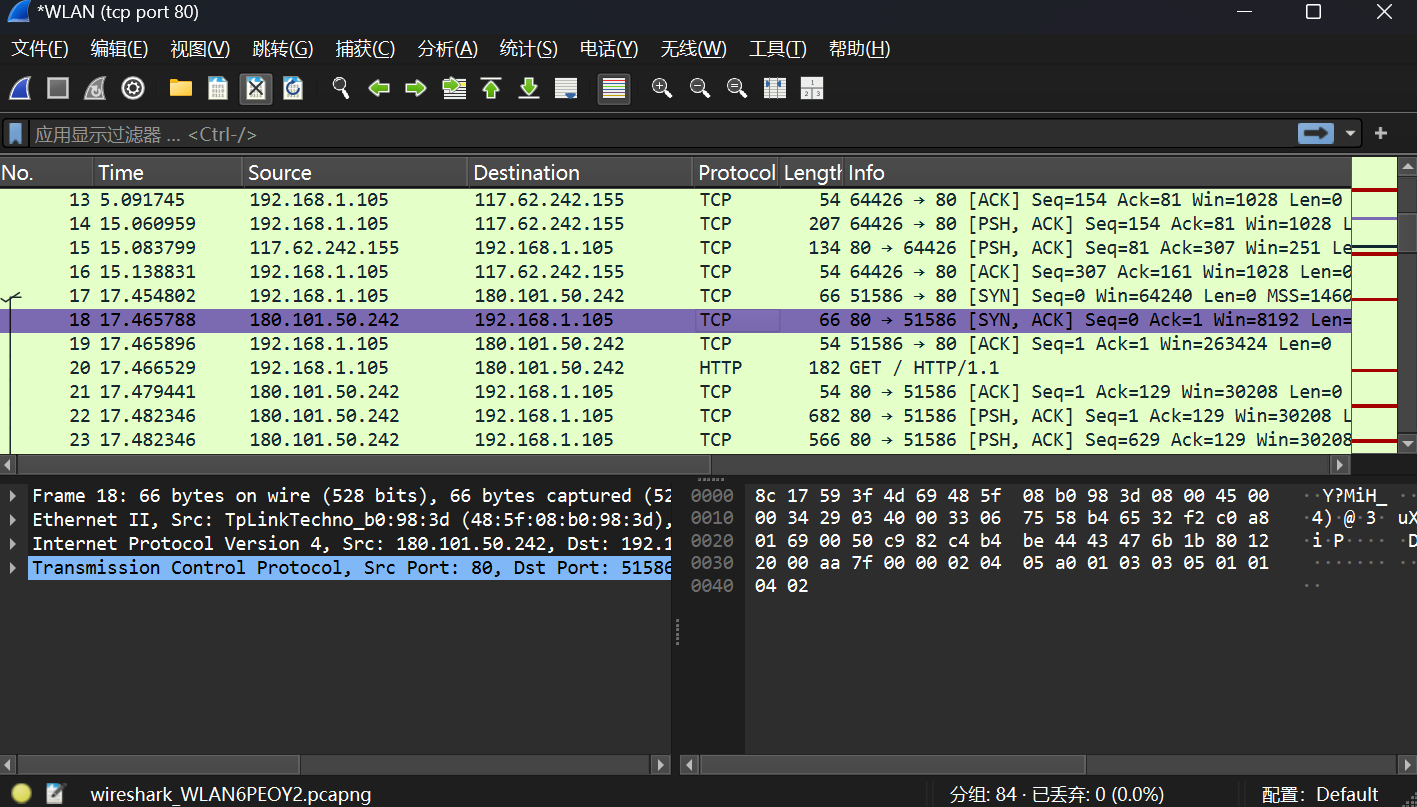
\includegraphics[width=11cm]{images/3. 捕获结果.png}
		\caption{捕获结果}
	\end{figure}
	
	\subsection{分析IPv4包并绘制报文结构、数据分析}
	
	选择捕获结果中的一个IP数据报,分析它的结构,如下图所示:
	
	\begin{figure}[H]
		\centering
		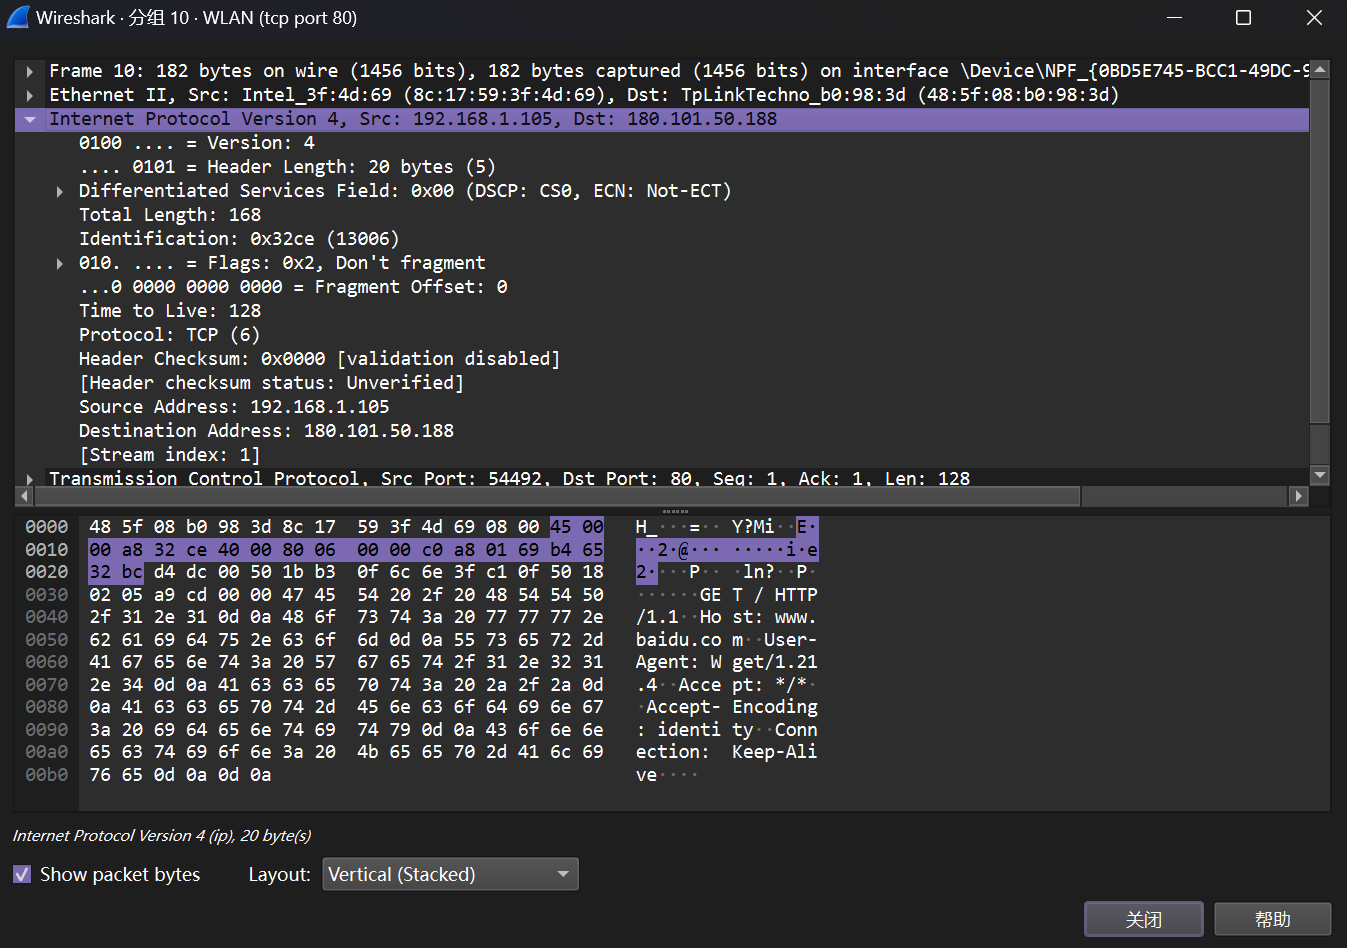
\includegraphics[width=11cm]{images/4. IPv4数据报结构.jpg}
		\caption{IPv4数据报结构}
	\end{figure}
	
	可以看到,第一个字段表示版本号(Version),长度为4bit,表示当前采用的IP协议版本号。一般是0100(IPv4)或者0110(IPv6)。
	
	\begin{figure}[H]
		\centering
		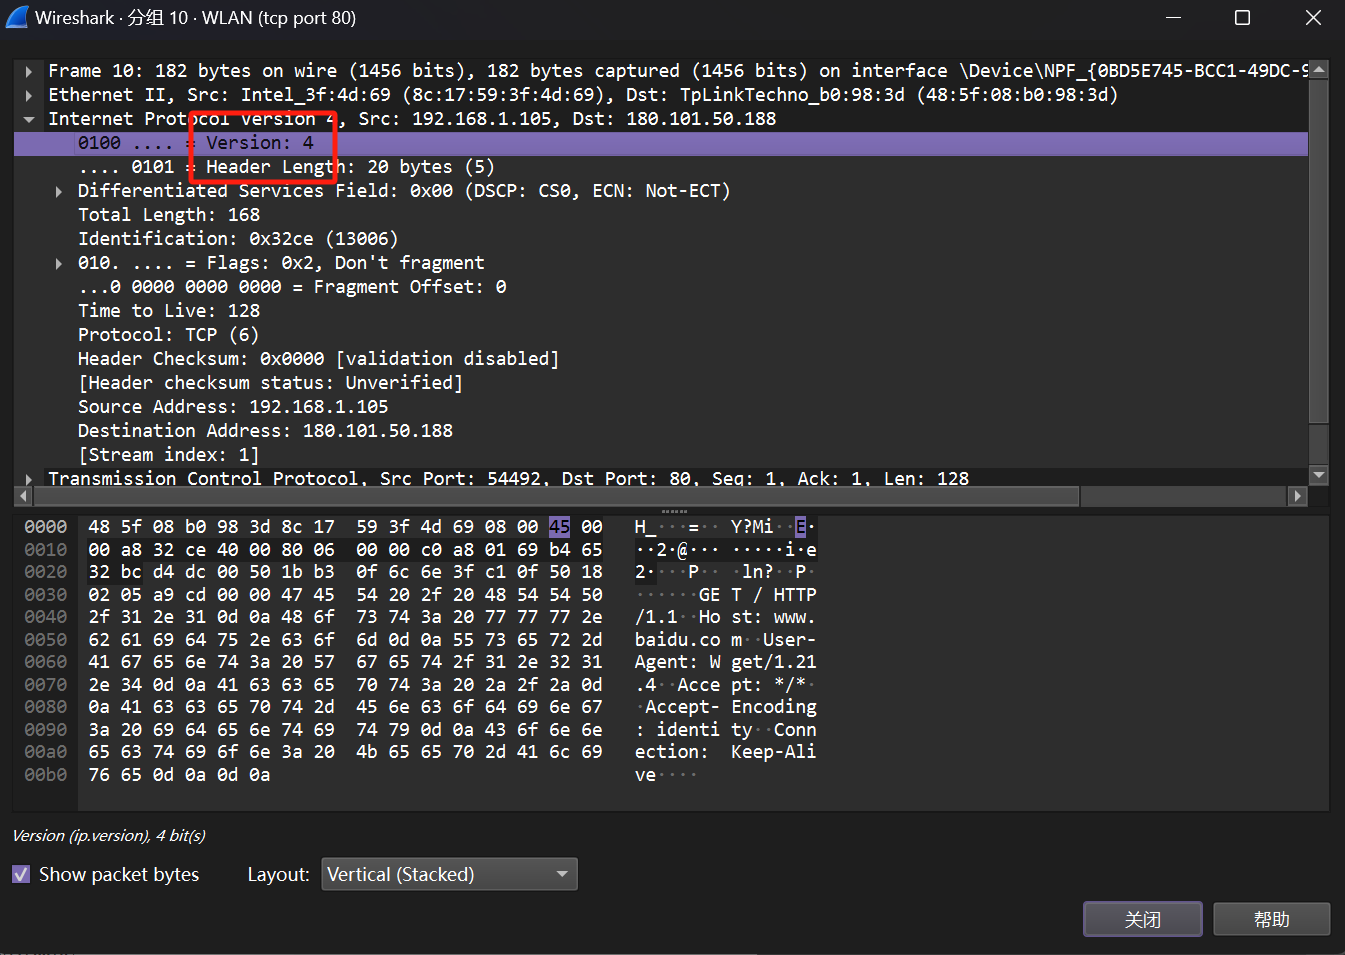
\includegraphics[width=11cm]{images/5. Version字段.jpg}
		\caption{Version字段}
	\end{figure}
	
	第二个字段表示首部长度,长度为 \texttt{4bit},表示IP报头的长度。在这个数据报中,首部长度为 \texttt{20 bytes}。
	
	\begin{figure}[H]
		\centering
		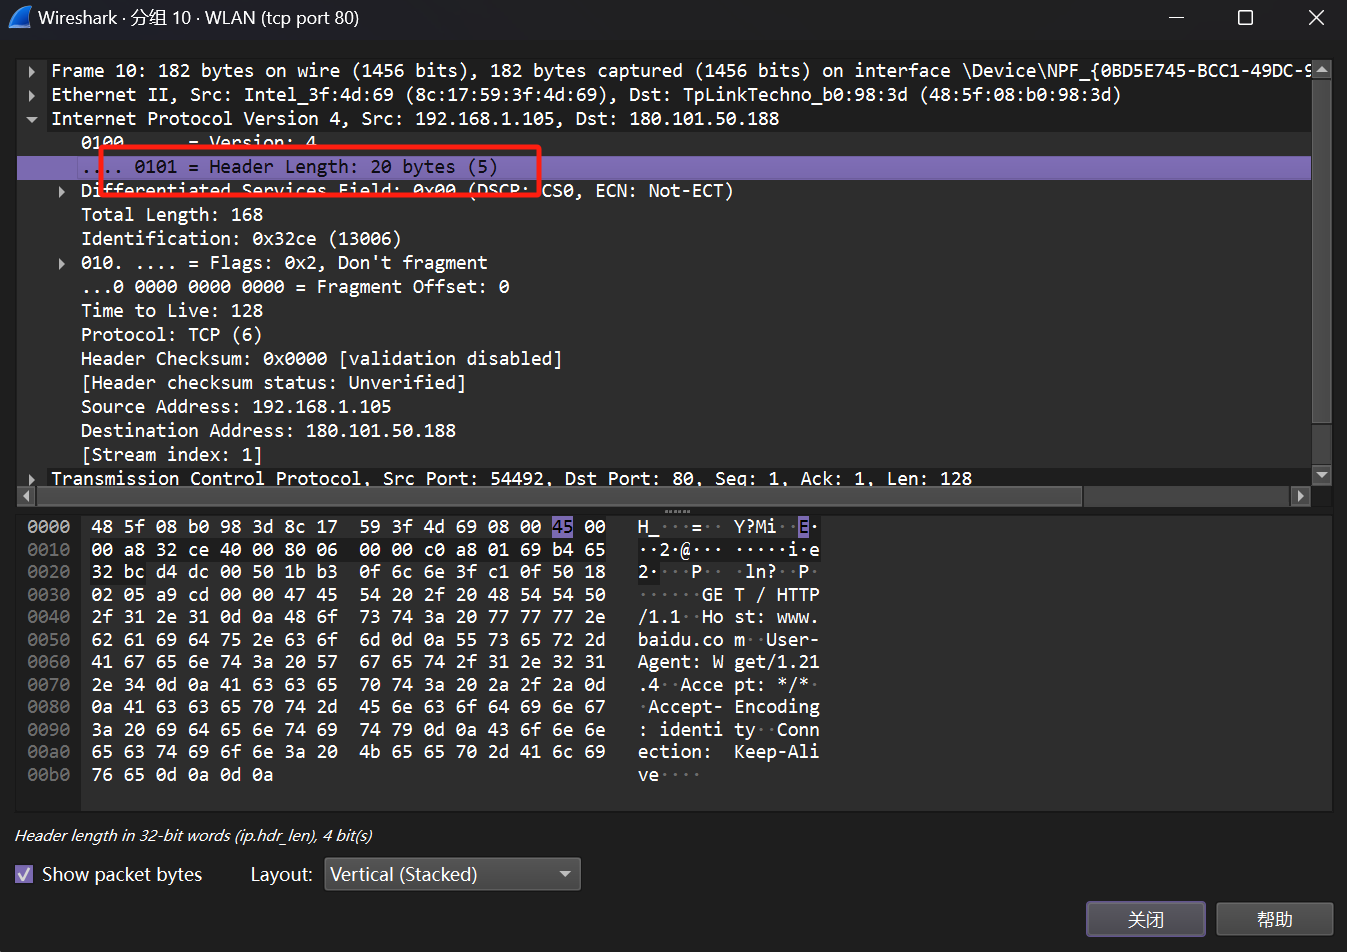
\includegraphics[width=11cm]{images/6. Header Length字段.jpg}
		\caption{Header Length字段}
	\end{figure}
	
	第三个字段表示区分服务,长度为 \texttt{1 byte},用于为不同的 \texttt{IP} 数据报定义不同的服务质量。
	
	\begin{figure}[H]
		\centering
		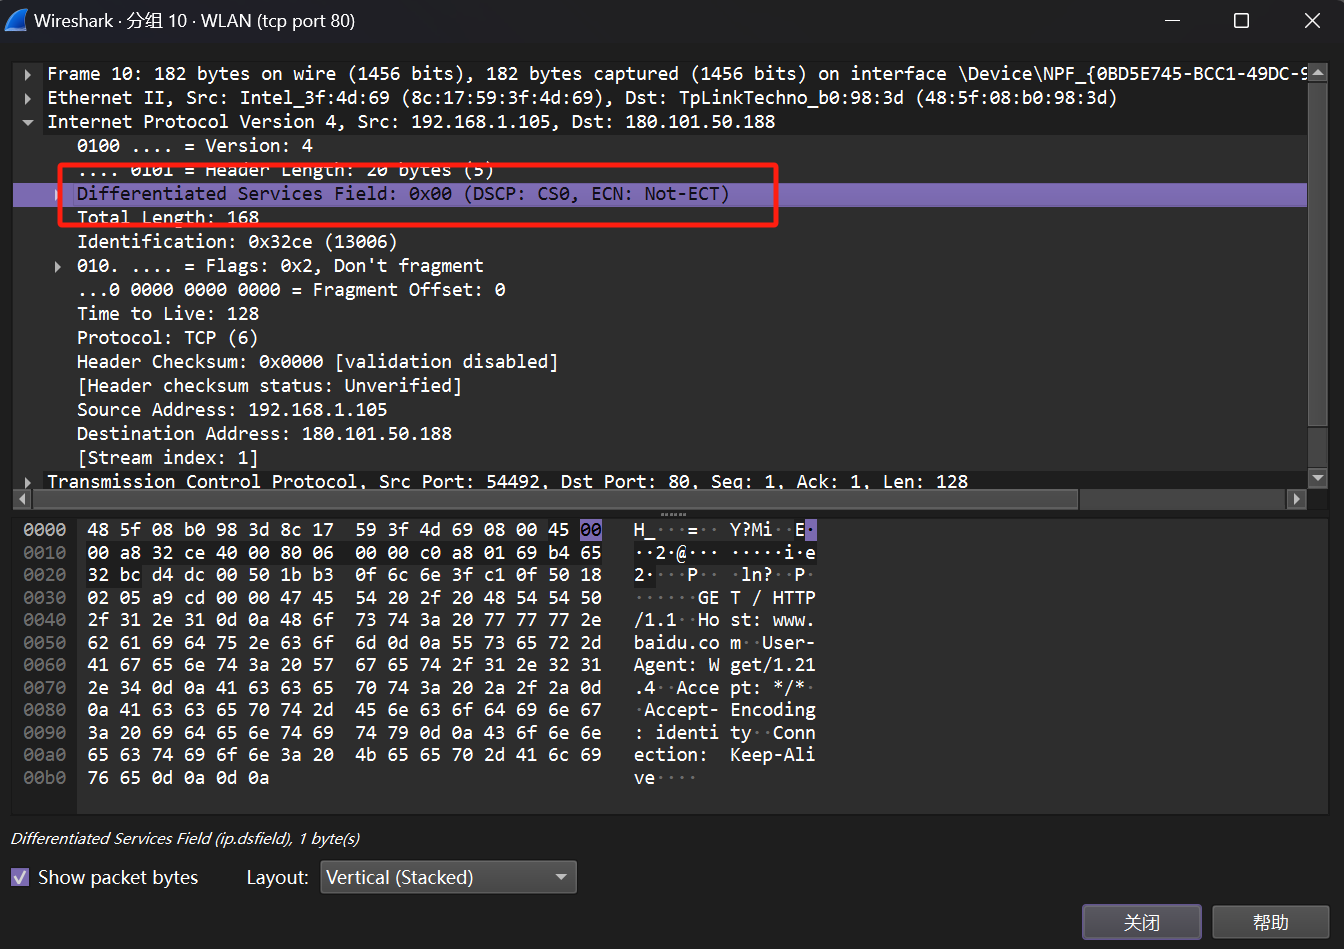
\includegraphics[width=11cm]{images/7. Differentiated Services 字段.jpg}
		\caption{Differentiated Services 字段}
	\end{figure}
	
	在这个字段中,包括:
	
	1) \texttt{DSCP},长度为 \texttt{6 bit},表示区分服务代码点,用于区分不同的服务质量; 
	
	2) \texttt{ECN},长度为 \texttt{2 bit},表示显式拥塞通知,用于指示网络拥塞。
	
	在这个数据报中, \texttt{DSCP} 的值为 \texttt{0x00},表示默认服务, \texttt{ECN} 的值为 \texttt{0x00},表示没有拥塞。
	
	\begin{figure}[H]
		\centering
		\begin{minipage}[b]{0.45\textwidth}
			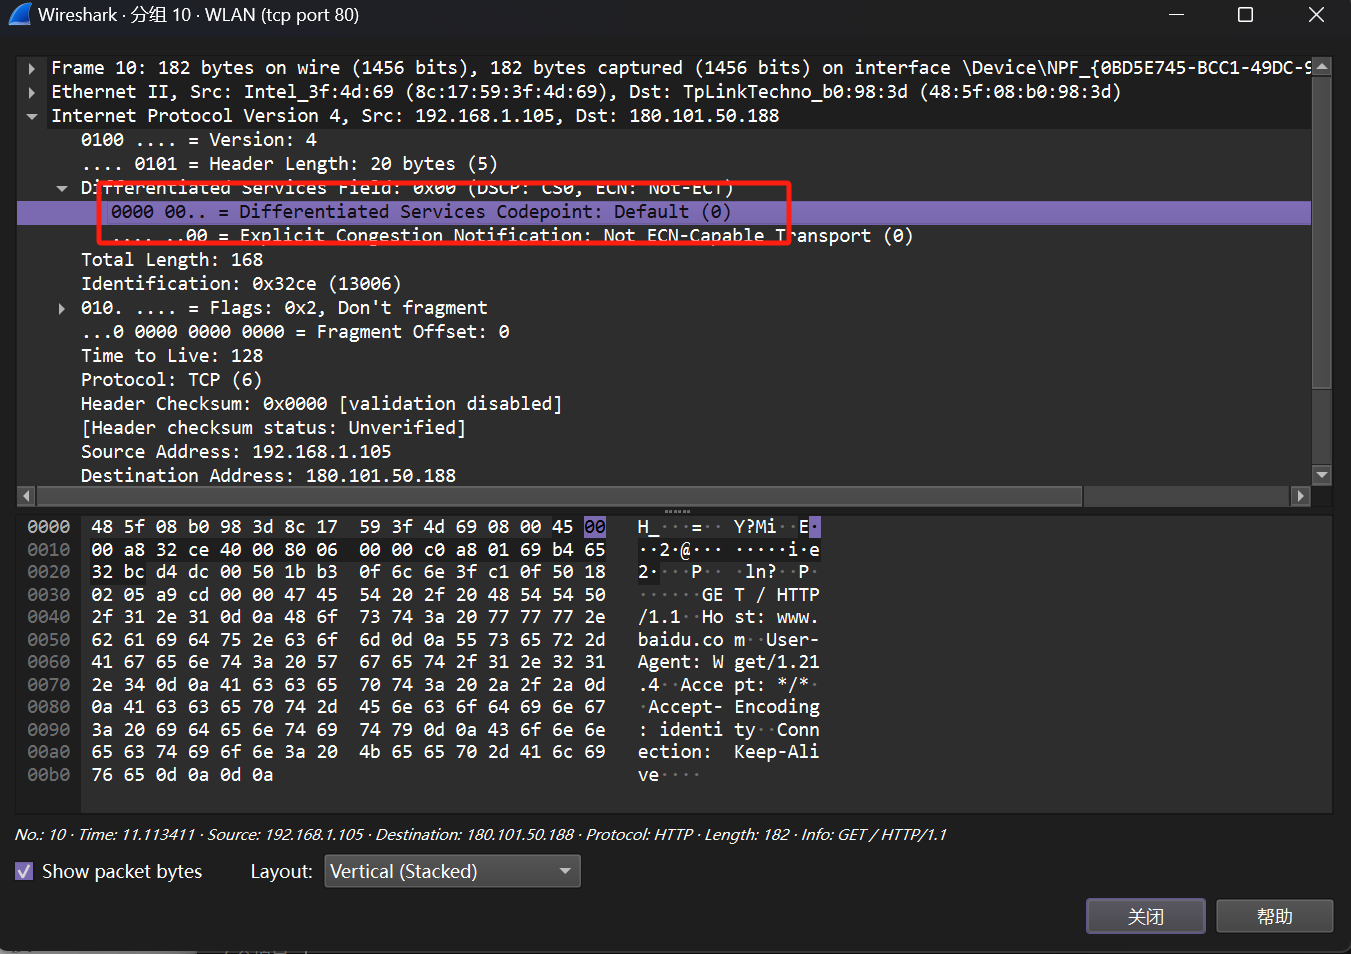
\includegraphics[width=\textwidth]{images/8. DSCP字段.jpg}
			\caption{TCP数据}
		\end{minipage}
		\hfill
		\begin{minipage}[b]{0.45\textwidth}
			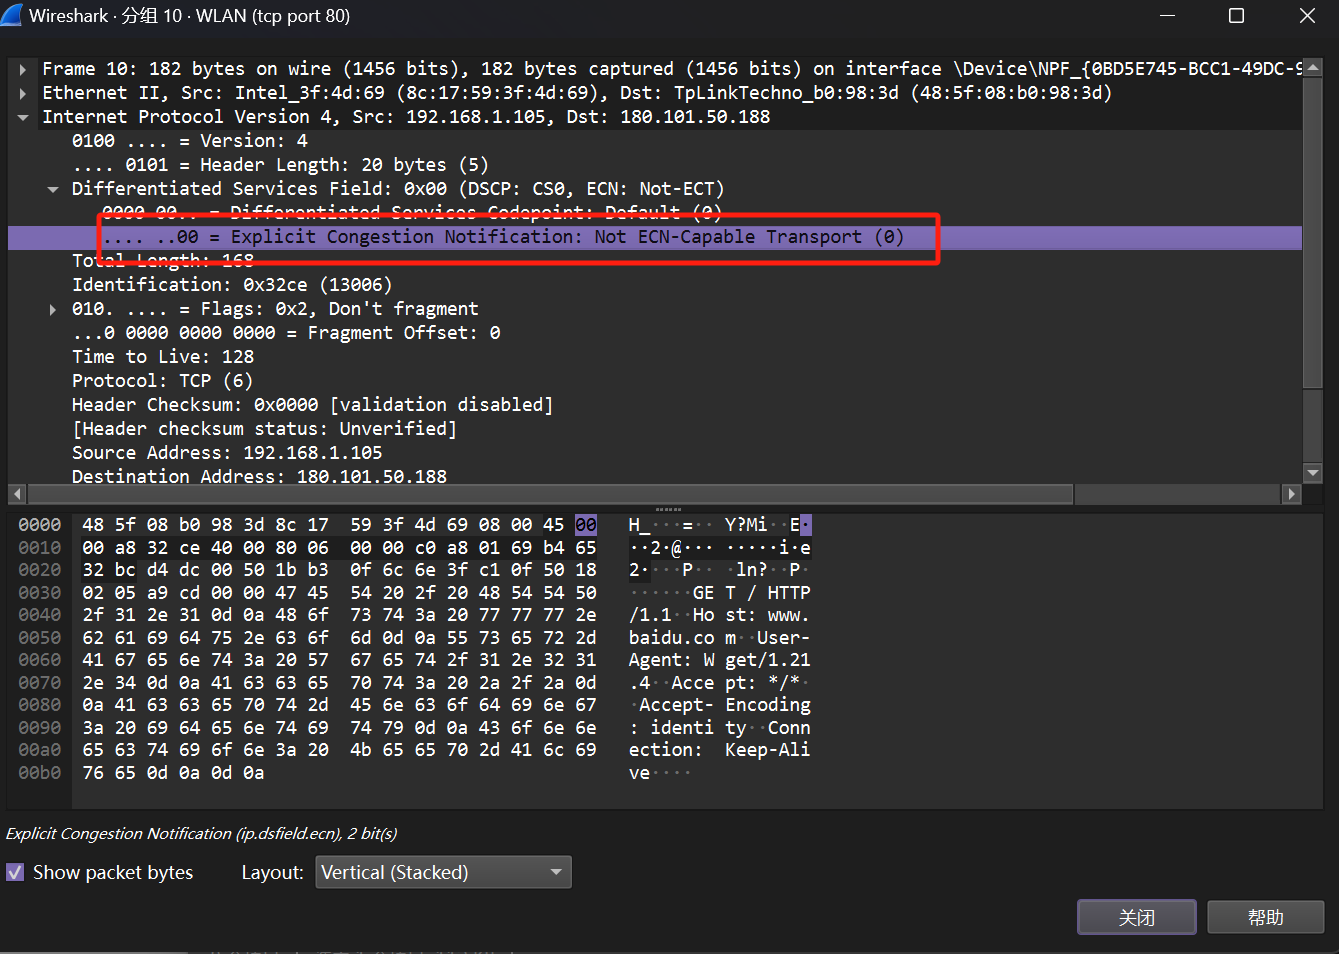
\includegraphics[width=\textwidth]{images/9. ECN字段.jpg}
			\caption{\texttt{HTTP数据}}
		\end{minipage}
	\end{figure}
	
	第四个字段指的是IP包的总长度,它占用\texttt{2 bytes}。这个字段以字节为单位,表示IP包的总长度,包括头部和数据部分。因此,IP包的最大长度被限制在\texttt{65,535 bytes}。数据包的有效载荷大小可以通过从IP包的总长度(\texttt{Total Length})中减去IP报头的长度(\texttt{Header Length})来计算。在当前的数据报中,记录的总长度为\texttt{168 bytes}。
	
	\begin{figure}[H]
		\centering
		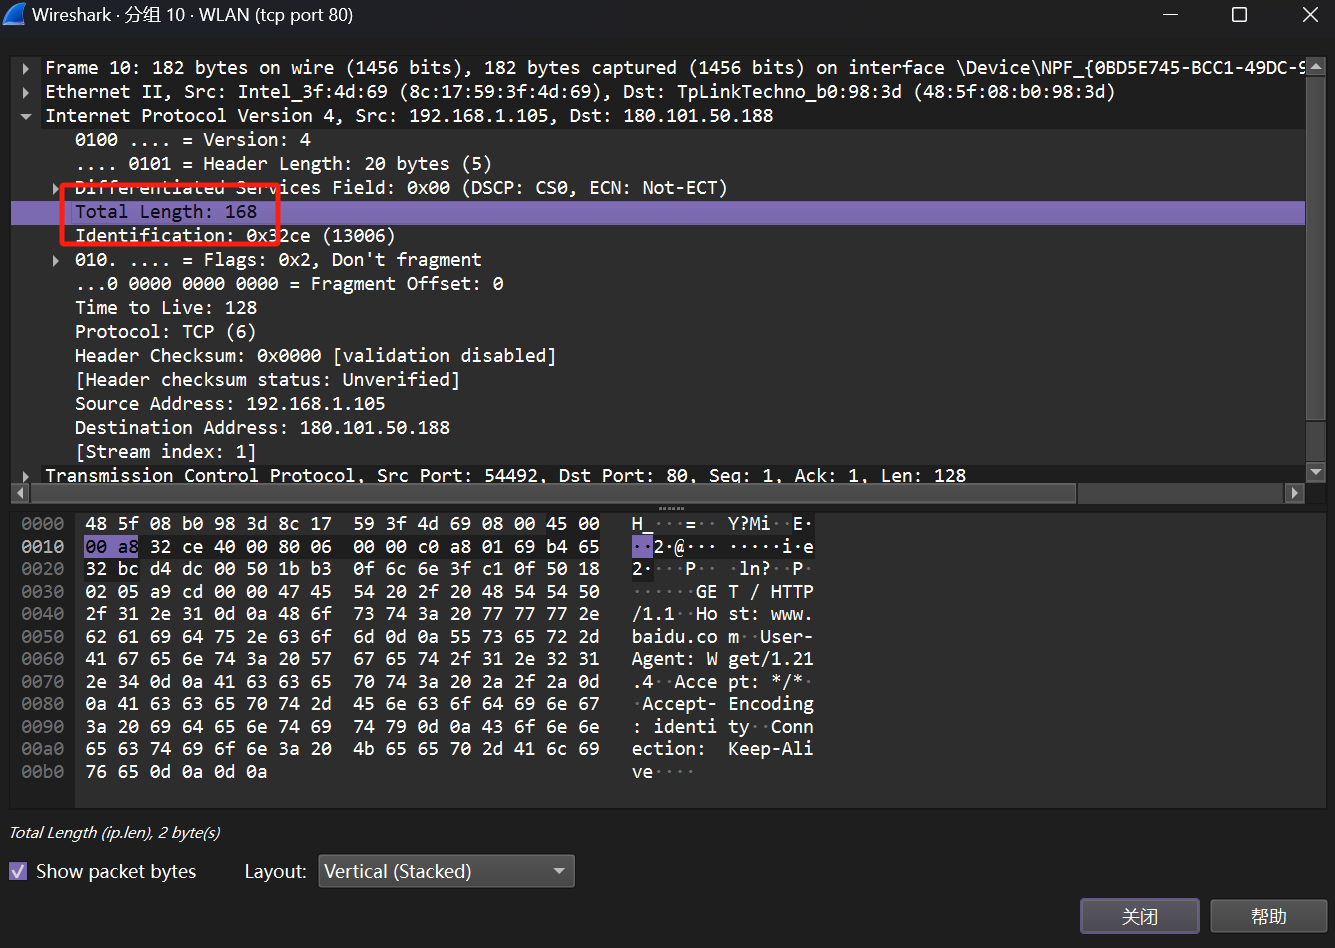
\includegraphics[width=11cm]{images/10. Total Length字段.jpg}
		\caption{Total Length字段}
	\end{figure}
	
	第五个字段是标识字段,它的长度为\texttt{2 bytes}。此标识字段与\texttt{Flags}字段和\texttt{Fragment Offset}字段协同工作,用于对较大的数据报执行分段操作。当路由器需要将一个较大的数据报分割成多个较小的片段以便传输时,所有这些片段都会分配相同的标识值。这样,接收端设备就可以识别出哪些片段属于同一个原始数据报。在本例中,数据报的标识字段值为\texttt{0x32ce}。
	
	\begin{figure}[H]
		\centering
		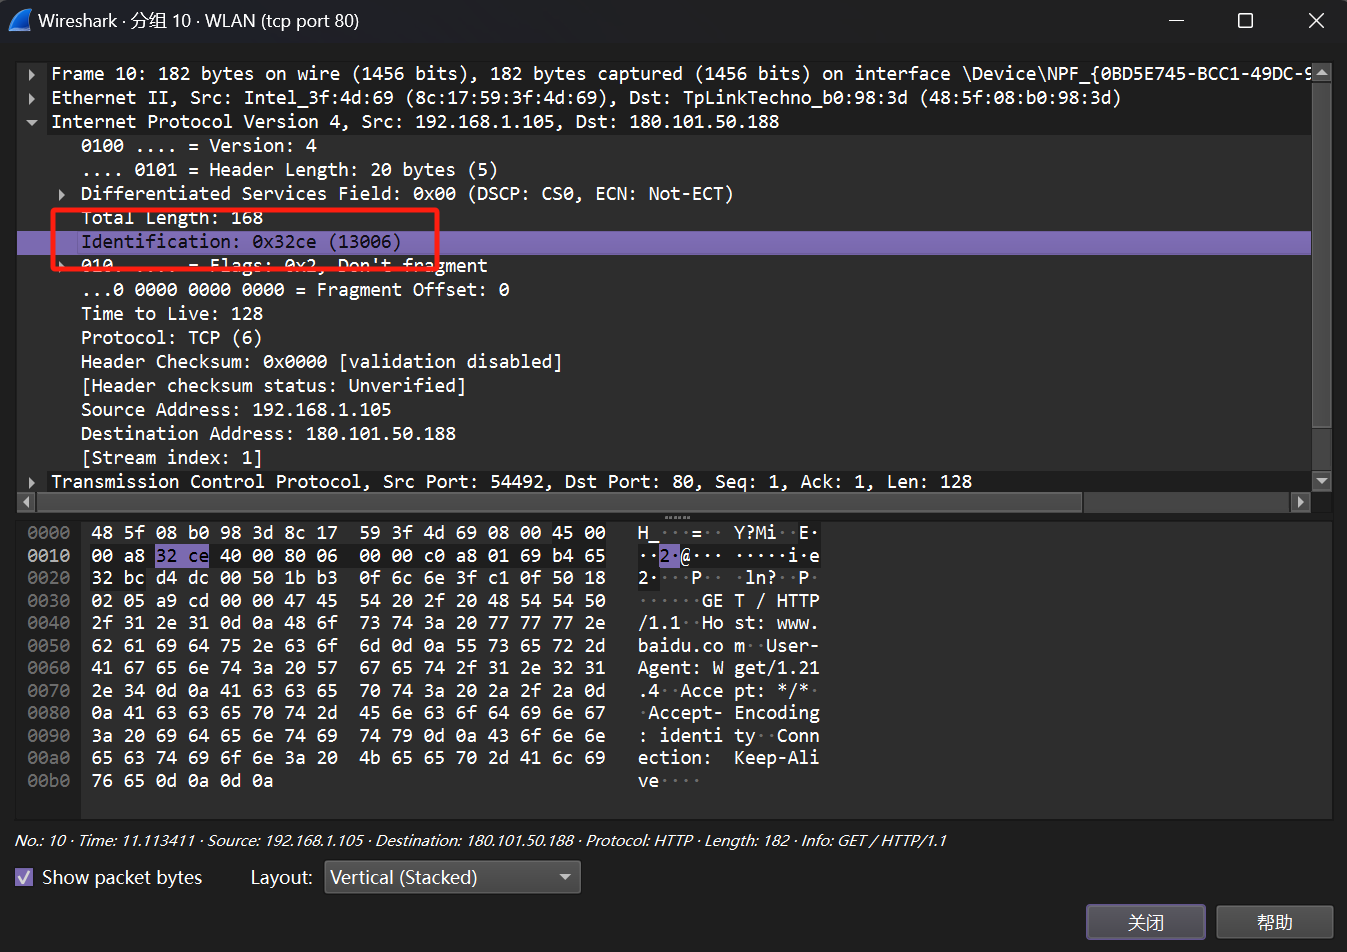
\includegraphics[width=11cm]{images/11. Identification字段.jpg}
		\caption{Identification字段}
	\end{figure}
	
	第六个字段被称为标志字段,其长度为\texttt{3 bits}。在这三个比特中,第一个比特是保留的,不用于任何特定的功能。第二个比特被称为\texttt{DF(Don't Fragment)}位。如果\texttt{DF}设置为1,这指示路由器不得对该数据报进行分段处理。在这种情况下,如果数据报的大小超过了网络的最大传输单元(MTU),路由器将丢弃该数据报,并发送一个错误信息回原始发送者。第三个比特是\texttt{MF(More Fragments)}位,当\texttt{MF}设置为1时,它表明在当前分段之后,还有更多的分段存在;而当\texttt{MF}设置为0时,这表示当前分段是数据报的最后一个分段。在所讨论的数据报中,标志字段的值为\texttt{0x02},这表明该数据报未被分段,并且没有后续的分段数据报。
	
	\begin{figure}[H]
		\centering
		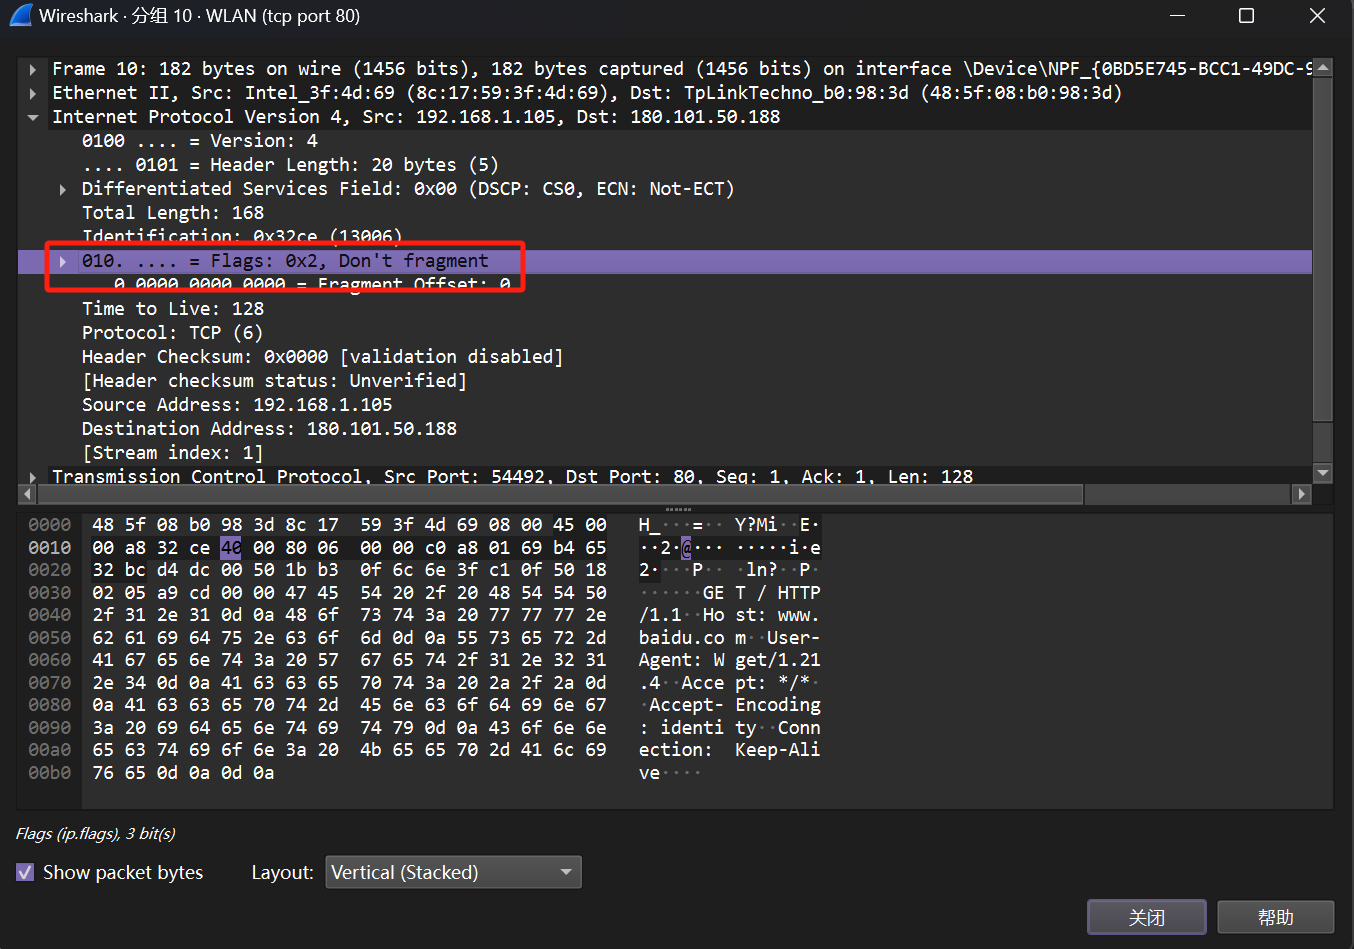
\includegraphics[width=11cm]{images/12. Flag字段.jpg}
		\caption{Flag字段}
	\end{figure}
	
	\begin{figure}[H]
		\centering
		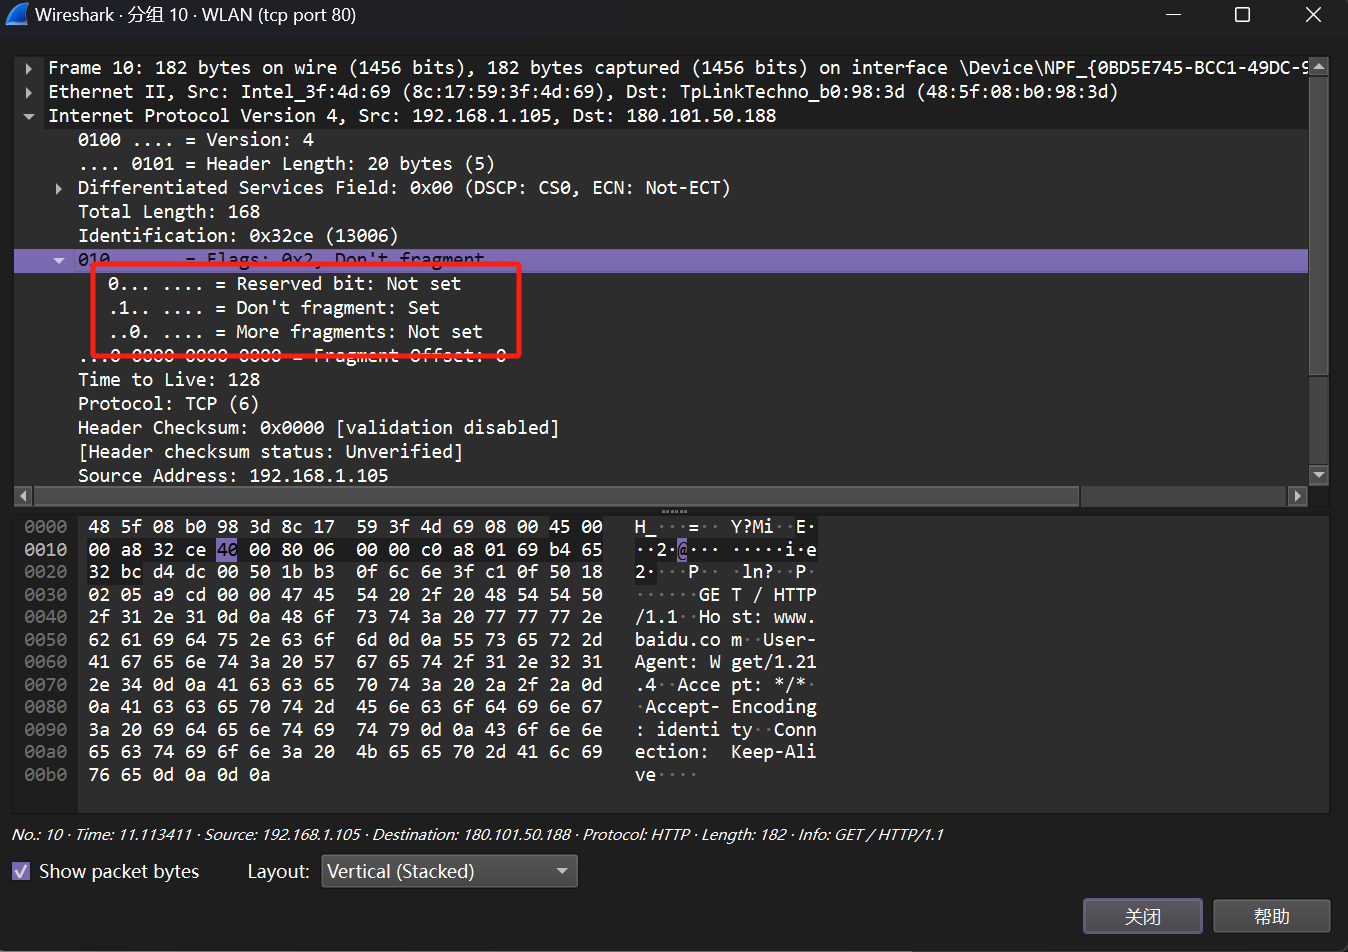
\includegraphics[width=11cm]{images/13. Flag字段内容.jpg}
		\caption{Flag字段内容}
	\end{figure}
	
	第七个字段定义为分片偏移,它的长度为\texttt{13 bits},并且以\texttt{8}字节为单位进行度量。分片偏移字段的功能是向接收端指明,当前分片在原始数据报中的位置。具体来说,它指示了分片数据部分相对于原始数据报数据起始部分的偏移量。这一信息对于接收端正确地重新组装原始IP数据包至关重要。在本数据报实例中,分片偏移量被设置为\texttt{0},意味着该分片是原始数据报的第一个分片,或者该数据报未被分片。
	
	\begin{figure}[H]
		\centering
		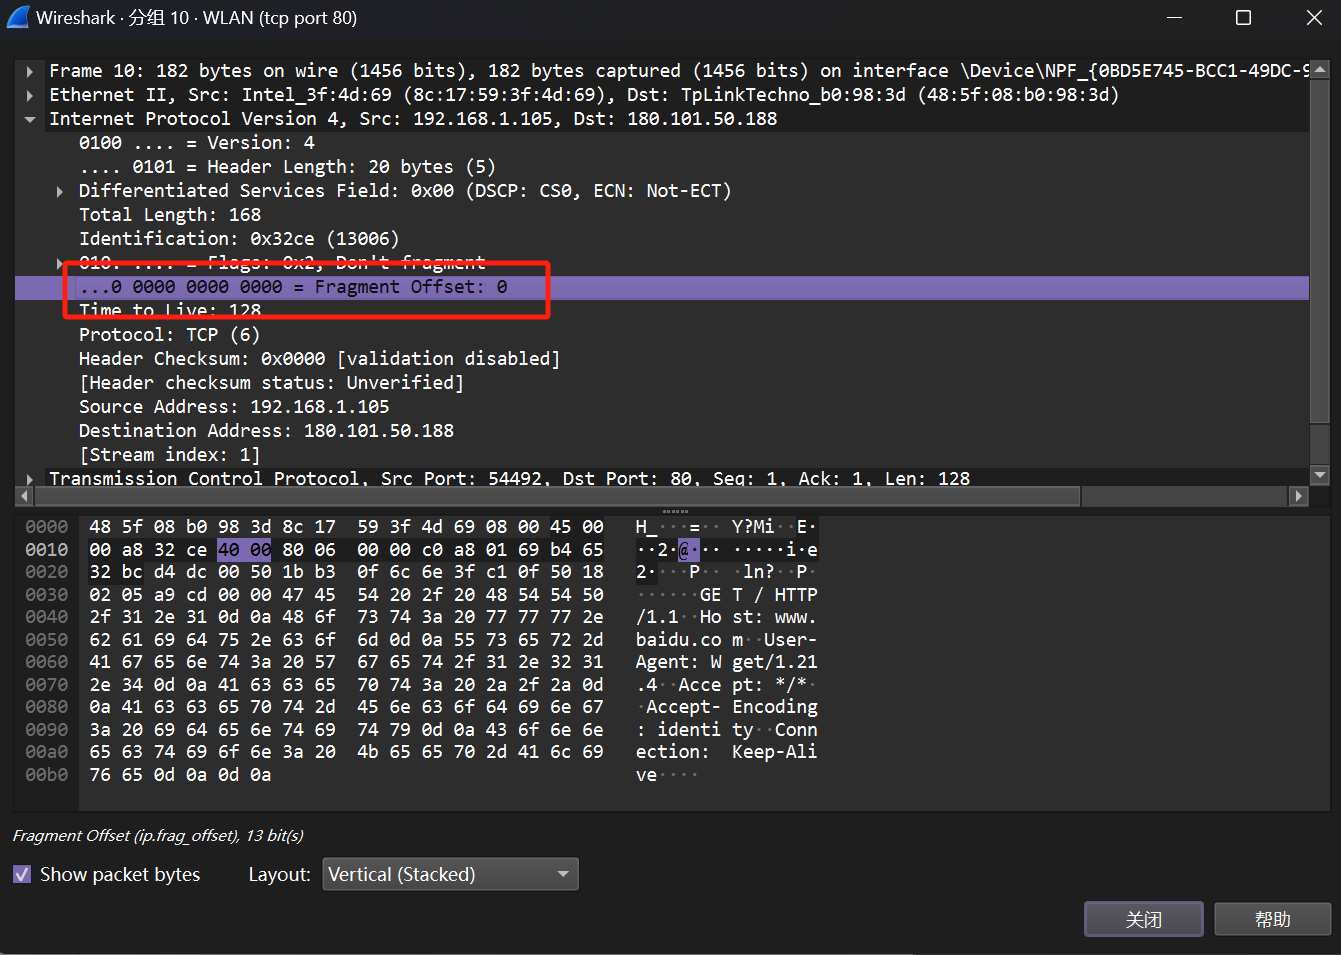
\includegraphics[width=11cm]{images/14. Fragment Offset字段.jpg}
		\caption{14. Fragment Offset字段.jpg}
	\end{figure}
	
	第八个字段是生存时间(Time to Live, TTL),其长度为\texttt{8 bits},并且以跳数(hops)为度量单位。此字段的设计初衷是为了限定数据报在网络中传输时所能经过的最大路由器数量。每当数据报通过一个三层设备,其TTL值将减少1。若TTL值降至0,该数据报将被网络设备丢弃,从而避免数据报在存在路由环路的网络中无限循环。在本数据报中,生存时间被设置为\texttt{128},这表明它在被丢弃前可以经过128个网络节点。
	
	\begin{figure}[H]
		\centering
		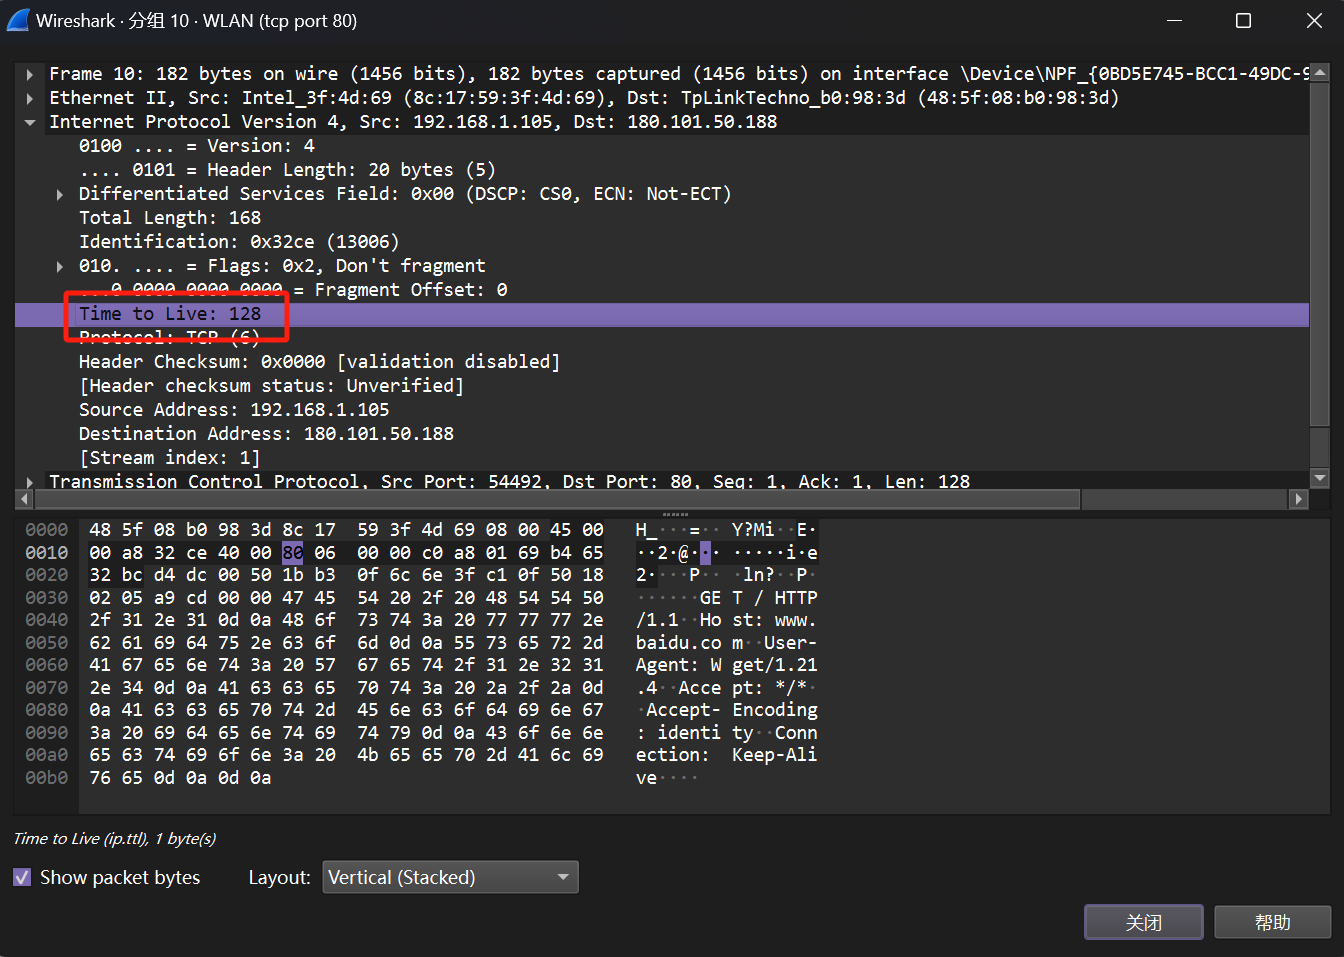
\includegraphics[width=10cm]{images/15. TTL字段.jpg}
		\caption{TTL字段}
	\end{figure}
	
	第九个字段被称为协议字段,占用\texttt{8 bits}。此字段用于指明数据报携带的上层协议类型。它允许接收端识别应该使用哪种协议来处理数据报的有效载荷。在本例中,数据报指定的协议为\texttt{TCP},其对应的值为\texttt{0x06},这表明数据报的上层协议是传输控制协议,通常用于提供可靠的、有序的和错误检测的数据传输。
	
	\begin{figure}[H]
		\centering
		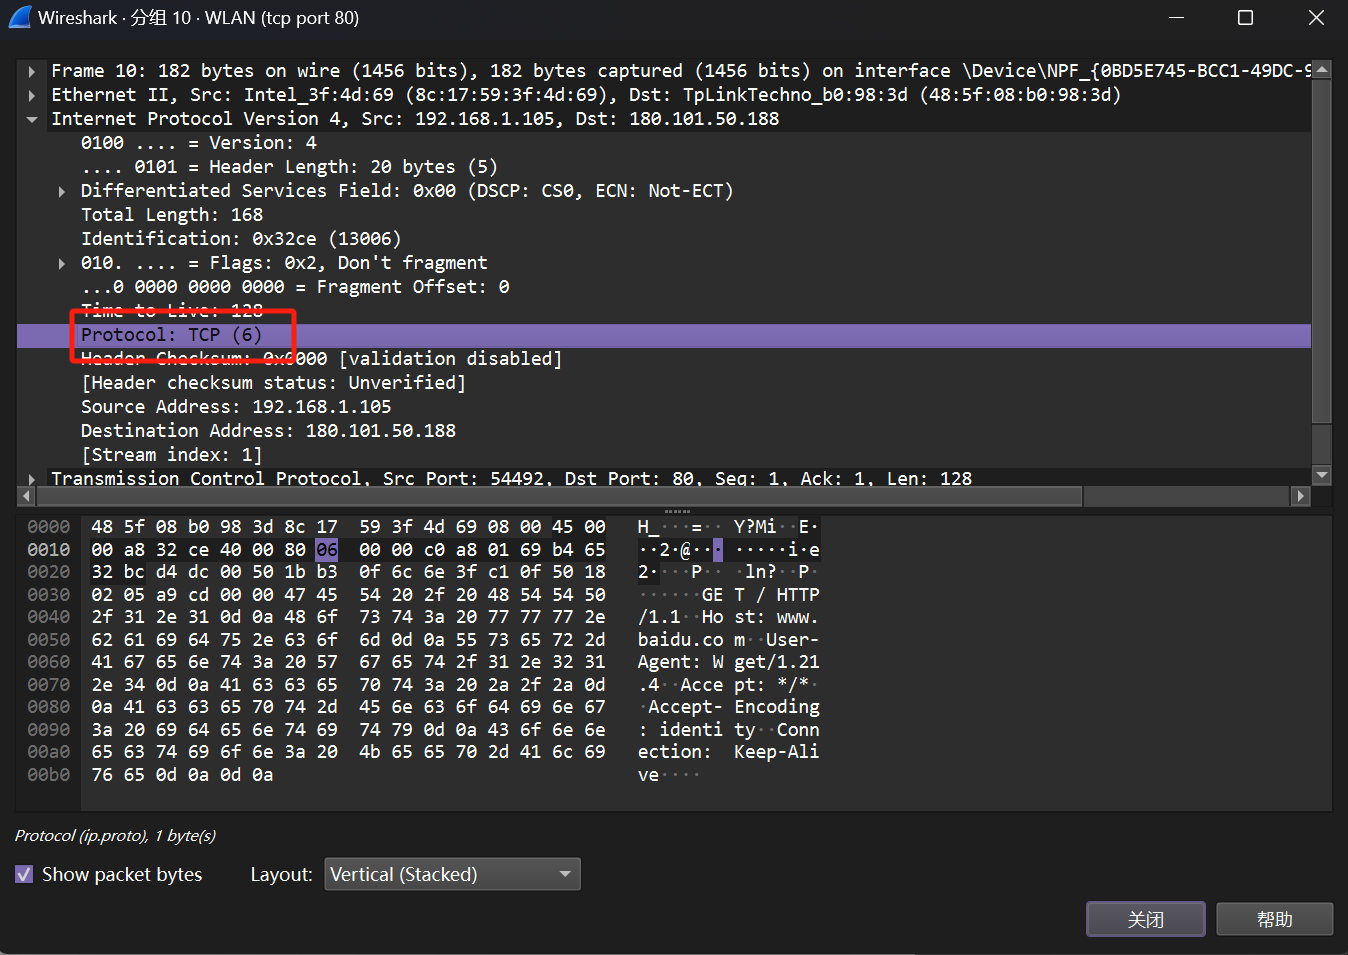
\includegraphics[width=10cm]{images/16. Protocal字段.jpg}
		\caption{Protocal字段}
	\end{figure}
	
	第十个字段是首部校验和,它的长度为\texttt{16 bits}。此字段专用于验证IP头部的完整性。校验和的计算不包括数据部分,仅涵盖IP包的头部信息。这是一种错误检测机制,用于确保在传输过程中头部信息未被损坏。在本数据报的案例中,记录的首部校验和值为\texttt{0x03d9}。
	
	\begin{figure}[H]
		\centering
		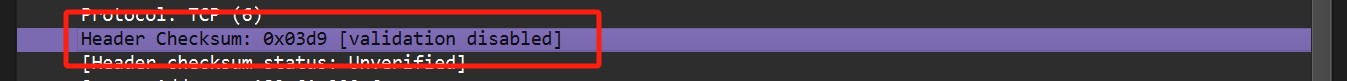
\includegraphics[width=10cm]{images/17. Header Checksum字段.jpg}
		\caption{Header Checksum字段}
	\end{figure}
	
	第十一个字段定义为源IP地址,占据\texttt{32 bits}的空间。这个字段用于记录发送方的网络地址,从而允许接收端识别数据包的起始点。在本次讨论的数据报中,源IP地址被指定为\texttt{192.168.1.105},这为网络通信提供了发送方的位置信息。
	
	\begin{figure}[H]
		\centering
		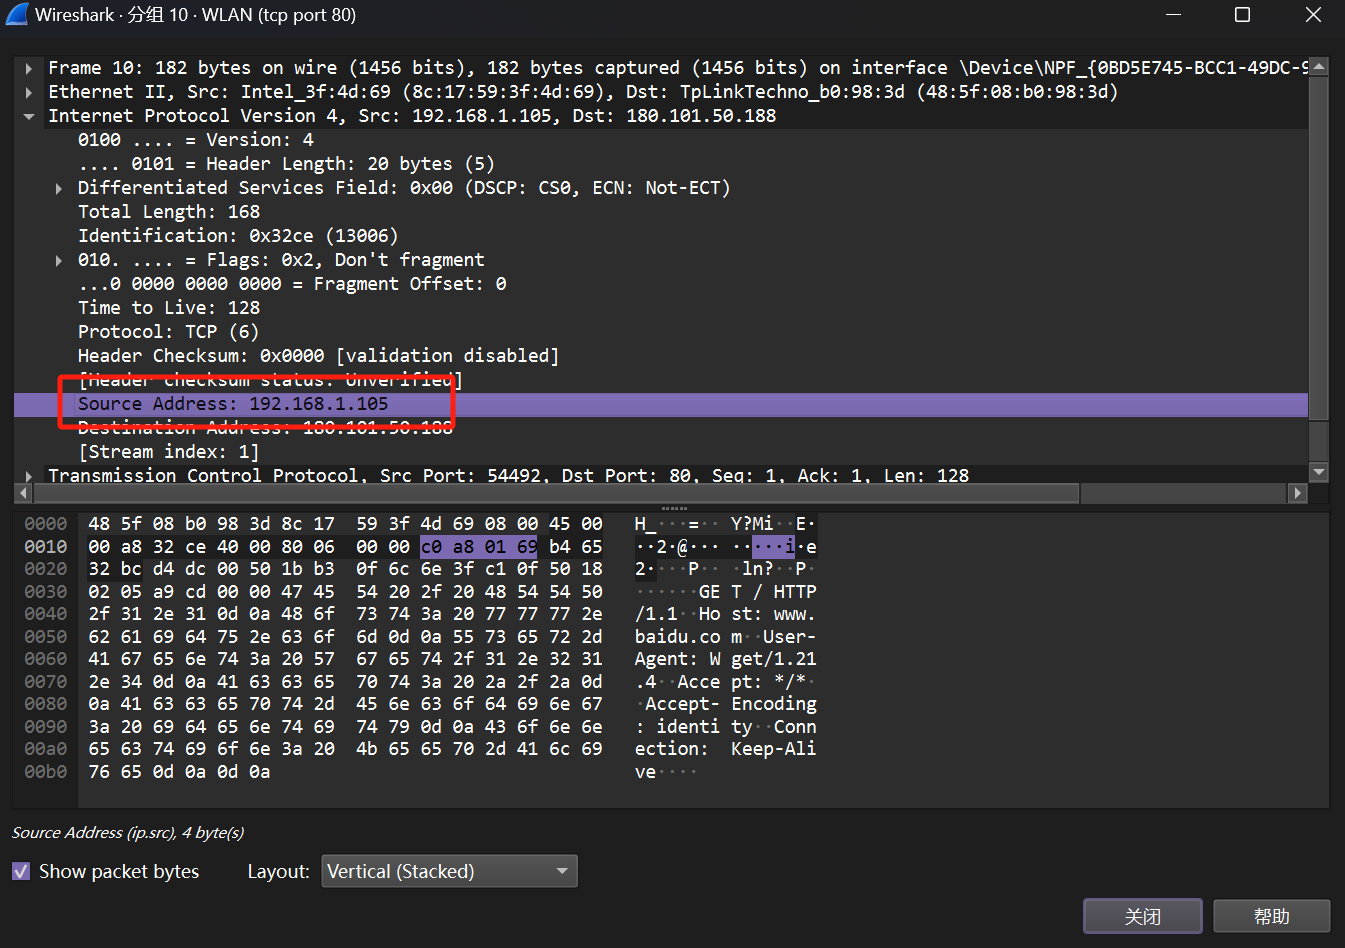
\includegraphics[width=10cm]{images/18. Source Address字段.jpg}
		\caption{Source Address字段}
	\end{figure}
	
	第十二个字段是目的IP地址,它的长度为\texttt{32 bits}。此字段用于标识数据包的接收方的网络地址,确保数据能够被正确地送达预定目的地。在本数据报实例中,目的IP地址被设置为\texttt{180.101.50.188},这明确了数据包的最终接收者。
	
	\begin{figure}[H]
		\centering
		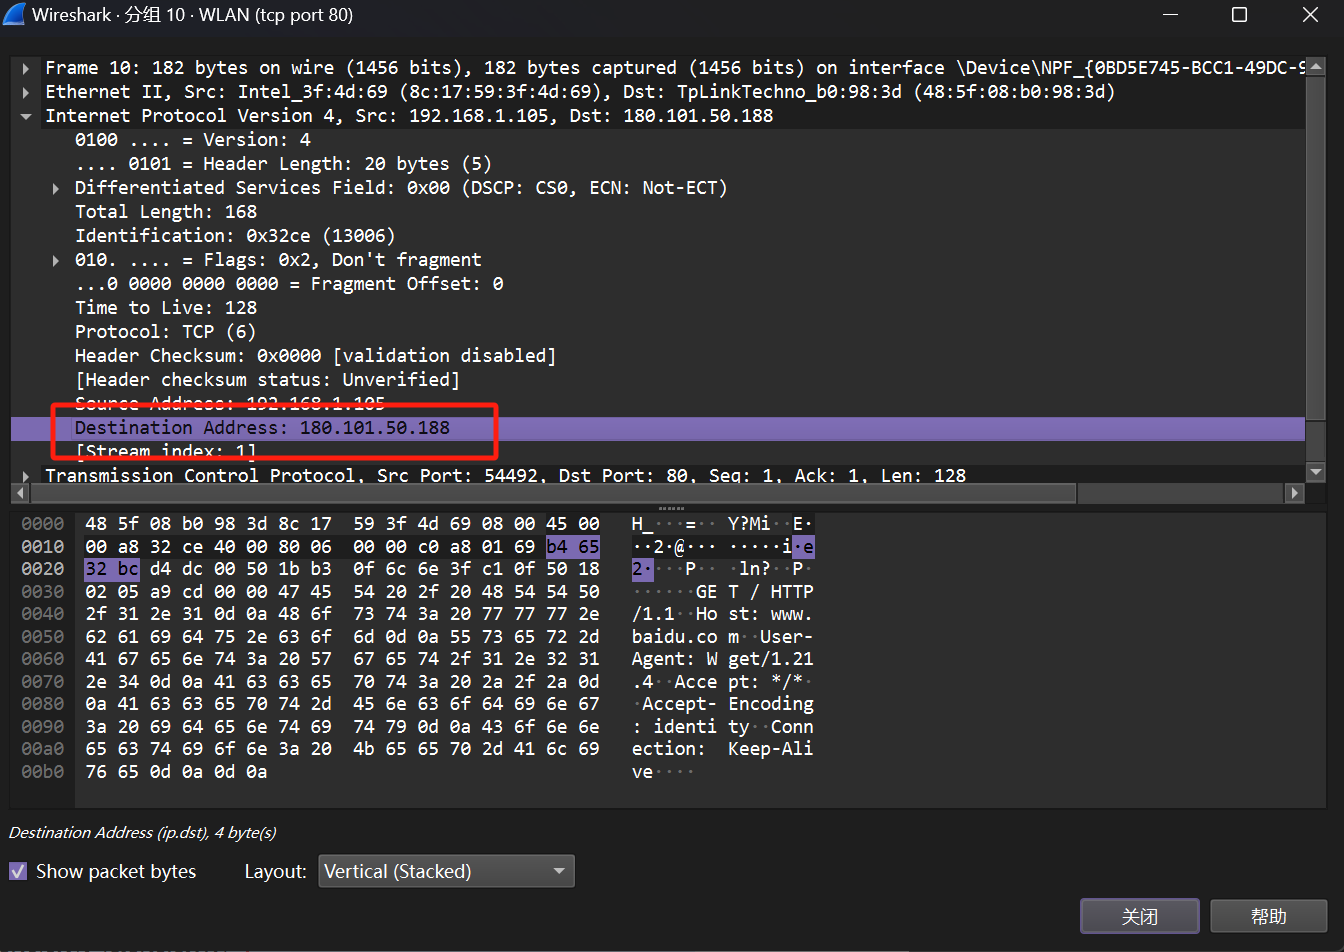
\includegraphics[width=10cm]{images/19. Destination Address字段.jpg}
		\caption{Destination Address字段}
	\end{figure}
	
	可以做出如下示意图来表示 \texttt{IP} 数据报的结构:
	
	\begin{figure}[H]
		\centering
		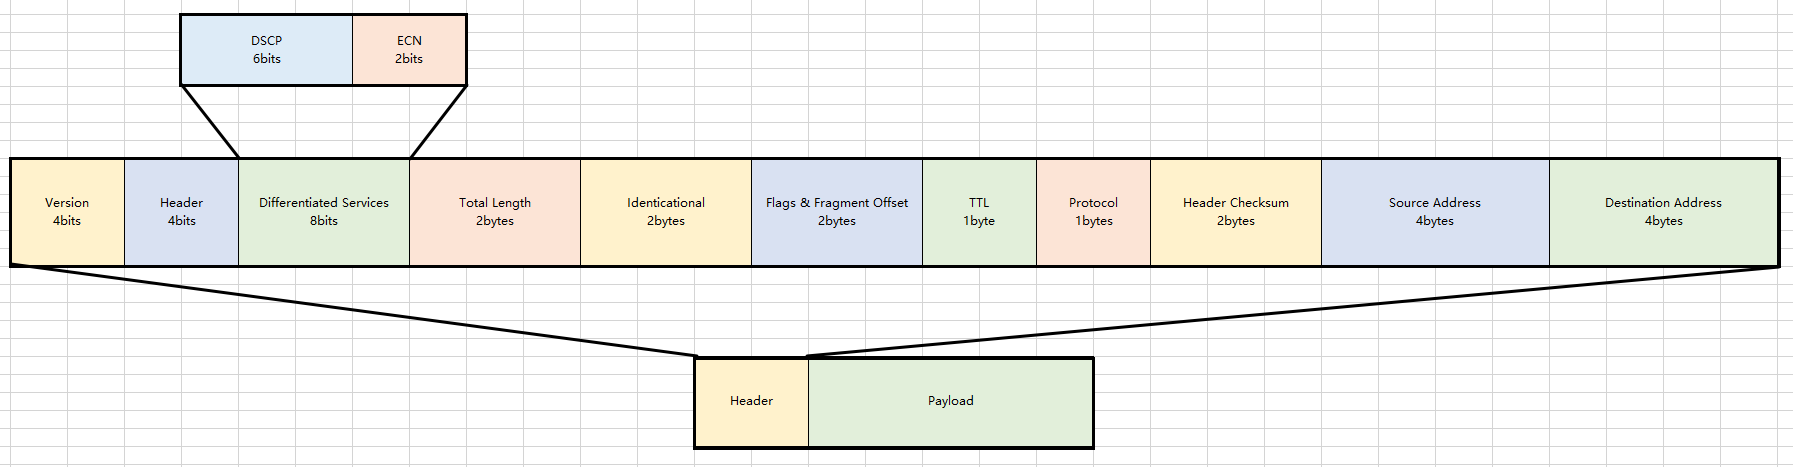
\includegraphics[width=18cm]{images/20. IP数据报结构示意图.jpg}
		\caption{IP数据报结构示意图}
	\end{figure}
	
	\subsection{回答问题}
	
	\begin{enumerate}[noitemsep]
		\item What are the IP addresses of your computer and the remote server?
		
		我的电脑的IP地址为 \texttt{192.168.1.105},远程服务器的IP地址为 \texttt{180.101.50.188}。
		\item Does the Total Length field include the IP header plus IP payload, or just the IP payload?
		
		\texttt{Total Length}字段包括\texttt{IP}报头和\texttt{IP}数据的总长度。
		\item How does the value of the Identification field change or stay the same for different packets? For instance, does it hold the same value for all packets in a TCP connection or does it differ for each packet? Is it the same in both directions? Can you see any pattern if the value does change?
		
		标识字段的值在不同的数据包中不同。在同一个 \texttt{TCP}连接中,标识字段的值不同。在同一个方向上,标识字段的值不同。在不同的方向上,标识字段的值不同。在这个数据报中,标识字段的值为 \texttt{0x32ce}。
		\item What is the initial value of the TTL field for packets sent from your computer? Is it the maximum possible value, or some lower value?
		
		我的电脑发送的数据包的生存时间字段的初始值为 \texttt{128},不是最大值。
		\item How can you tell from looking at a packet that it has not been fragmented? Most often IP packets in normal operation are not fragmented. But the receiver must have a way to be sure. Hint: you may need to read your text to confirm a guess.
		
		如果一个数据包没有被分段,那么它的标志字段的 \texttt{DF}位为 \texttt{1},且标志字段的 \texttt{MF}位为 \texttt{0}。
		\item What is the length of the IP Header and how is this encoded in the header length field? Hint: notice that only 4 bits are used for this field, as the version takes up the other 4 bits of the byte. You may guess and check your text.
		
		\texttt{IP}报头的长度为 \texttt{20 bytes},版本号和首部长度字段共占 \texttt{8 bits},其中版本号占 \texttt{4 bits},首部长度占 \texttt{4 bits}。
	\end{enumerate}
	
	\subsection{Internet Path}
	
	在命令行下使用tracert命令,查看到达\texttt{www.baidu.com}的路由路径。根据输出画出网络路径。
	
	\begin{figure}[H]
		\centering
		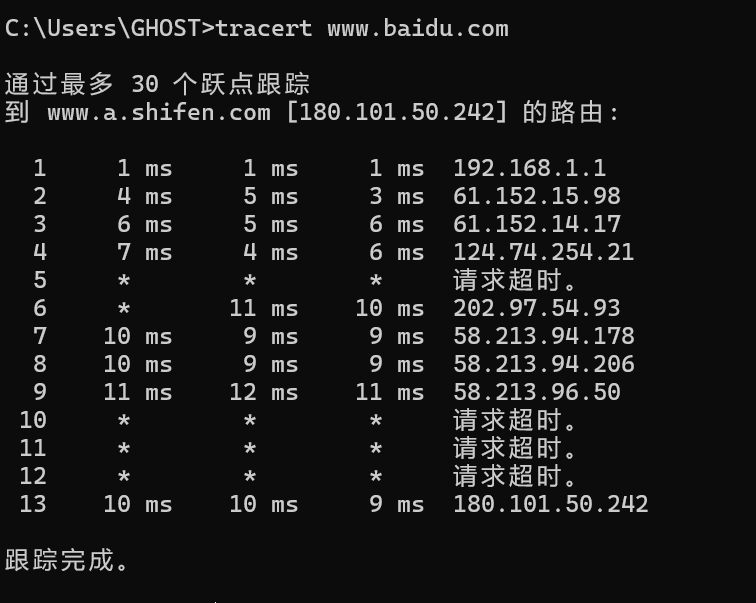
\includegraphics[width=10cm]{images/21. tracert命令输出.jpg}
		\caption{tracert命令输出}
	\end{figure}
	
	画出网络路径图如下:
	
	\begin{figure}[H]
		\centering
		\begin{tikzpicture}[node distance=0.5cm, >=Stealth, rect/.style={draw, minimum width=2cm, minimum height=1cm, text centered}]
			
			% Draw rectangles
			\node (me) [rect] {本机};
			\node (1) [rect, below=of me] {192.168.1.1};
			\node (2) [rect, below=of 1] {61.152.15.98};
			\node (3) [rect, below=of 2] {61.152.14.17};
			\node (4) [rect, below=of 3] {124.74.254.21};
			\node (5) [rect, below=of 4] {*};
			\node (6) [rect, below=of 5] {202.97.54.93};
			\node (7) [rect, below=of 6] {58.213.94.178};
			\node (8) [rect, right=of 7] {58.213.94.206};
			\node (9) [rect, above=of 8] {58.213.96.50};
			\node (10) [rect, above=of 9] {*};
			\node (11) [rect, above=of 10] {*};
			\node (12) [rect, above=of 11] {*};
			\node (13) [rect, above=of 12] {180.101.50.242};
			
			% Draw arrows
			\draw[->] (me.south) -- (1.north);
			\draw[->] (1.south) -- (2.north);
			\draw[->] (2.south) -- (3.north);
			\draw[->] (3.south) -- (4.north);
			\draw[->] (4.south) -- (5.north);
			\draw[->] (5.south) -- (6.north);
			\draw[->] (6.south) -- (7.north);
			\draw[->] (7.east) -- (8.west);
			\draw[->] (8.north) -- (9.south);
			\draw[->] (9.north) -- (10.south);
			\draw[->] (10.north) -- (11.south);
			\draw[->] (11.north) -- (12.south);
			\draw[->] (12.north) -- (13.south);
			
		\end{tikzpicture}
		\caption{网络路径图}
		\label{fig:22}
	\end{figure}
	
	\subsection{计算\texttt{checksum}}
	
	\texttt{IP}报头的校验和可以用来验证一个数据包是否正确。
	我们再选择一个新的 \texttt{IP}报文,计算它的 \texttt{checksum}。
	
	\begin{figure}[H]
		\centering
		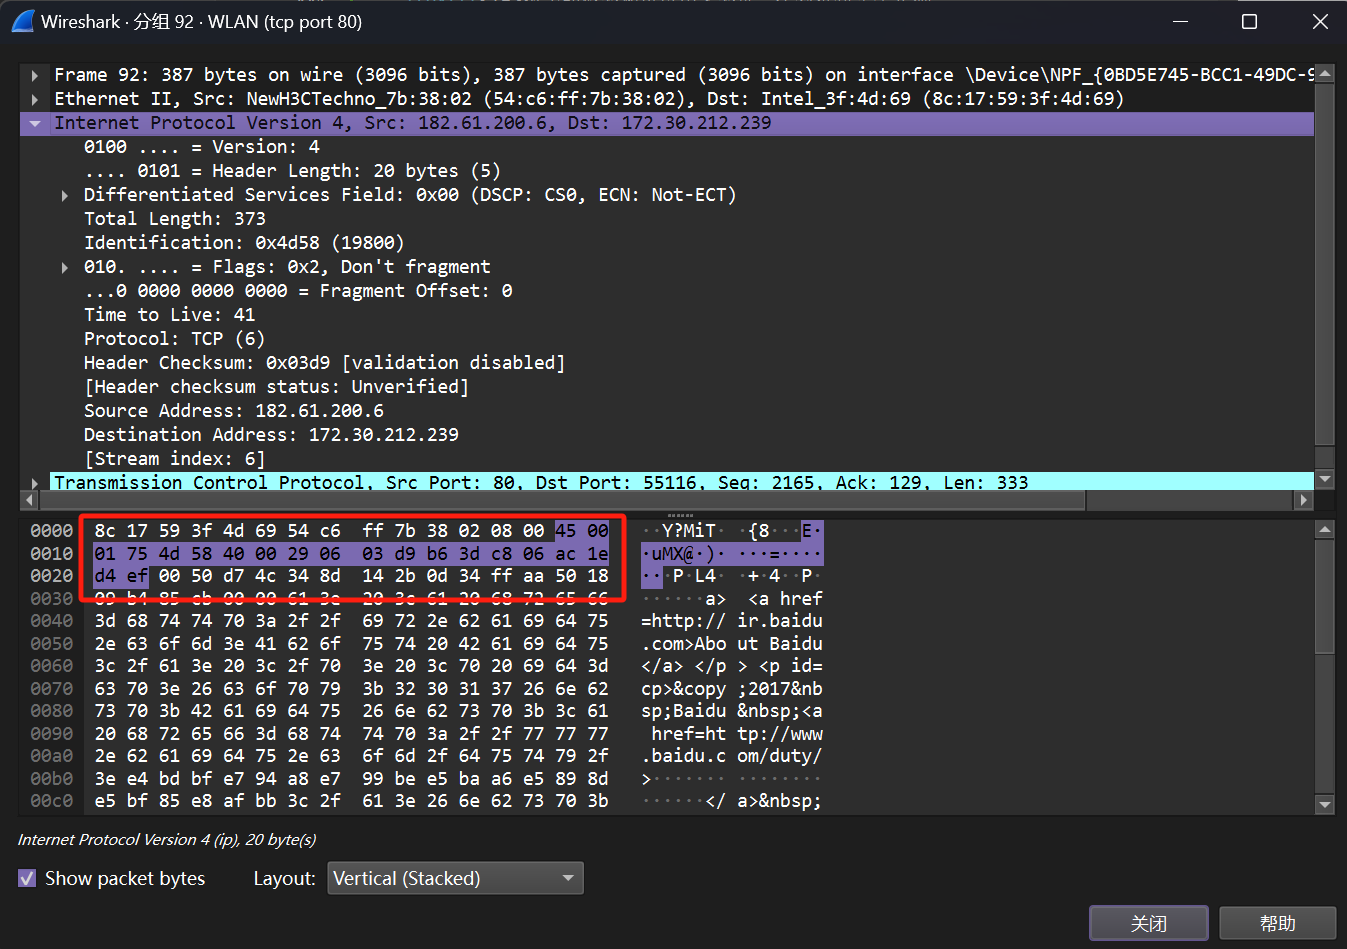
\includegraphics[width=8cm]{images/22. 选择一个IPv4进行计算.jpg}
		\caption{选择一个IPv4进行计算}
	\end{figure}
	
	将其校验和字段置为0后,数据如下:
	45 00 01 75 4d 58 40 00 29 06 00 00 b6 3d c8 06 ac 1e d4 ef
	
	将其分为两个字节一组,进行二进制求和,再将最高位的进位加到低16位,得到的结果如下:
	
	\begin{lstlisting}[numbers=none]
		     45 00 
		+    01 75
		+    4d 58 
		+    40 00 
		+    29 06
		+    b6 3d
		+    c8 06
		+    ac 1e
		+    d4 ef
		--------------
		   3 fc 23
		+        3
		--------------
		     fc 26
	\end{lstlisting}
	
	取反后,得到 \texttt{checksum}为 \texttt{0x03d9},与原数据报中的 \texttt{checksum}字段相同。
	
	\begin{lstlisting}[numbers=none]
		  ff ff
		- fc 26
		-----------
		  03 d9
	\end{lstlisting}
	
	\subsection{问题讨论}
	
	\begin{enumerate}[noitemsep]
		\item Read about and experiment with IPv6. Modern operating systems already include support for IPv6so you may be able to capture IPv6 traffic on your network. You can also “join the IPv6'backbone by tunneling to an IPv6 provider.
		
		\texttt{IPv6}是\texttt{IP}协议的下一代协议,它的主要特点是地址空间更大,报头更简单,安全性更好,支持多播和组播,支持流量标签,支持流量优先级,支持更多的选项和扩展,支持更多的协议。现代操作系统已经支持\texttt{IPv6},可以在网络上捕获\texttt{IPv6}流量。也可以通过隧道连接到\texttt{IPv6}提供者。
		
		我们使用 \texttt{Wireshark}捕获\texttt{IPv6}数据包.
		
		在 \texttt{Wireshark}的筛选器中输入 \texttt{ipv6},可以看到捕获到的\texttt{IPv6}数据包。
		
		\begin{figure}[H]
			\centering
			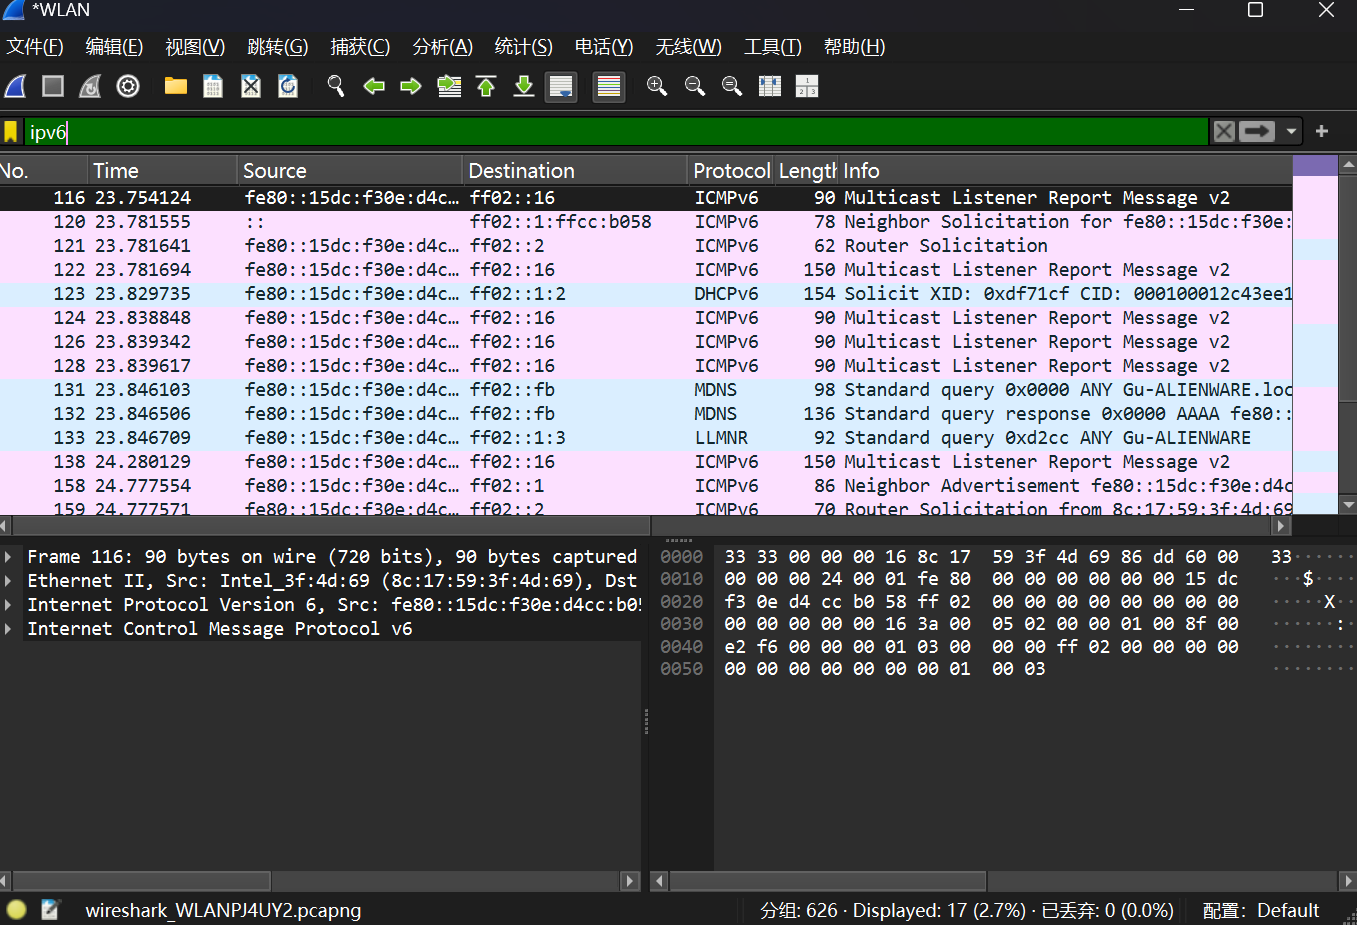
\includegraphics[width=11cm]{images/23. Wireshark捕获IPv6数据包.jpg}
			\caption{\texttt{Wireshark}捕获\texttt{IPv6}数据包}
			\label{fig:23}
		\end{figure}
		
		选择其中的一个数据包,可以看到其结构如下:
		
		\begin{figure}[H]
			\centering
			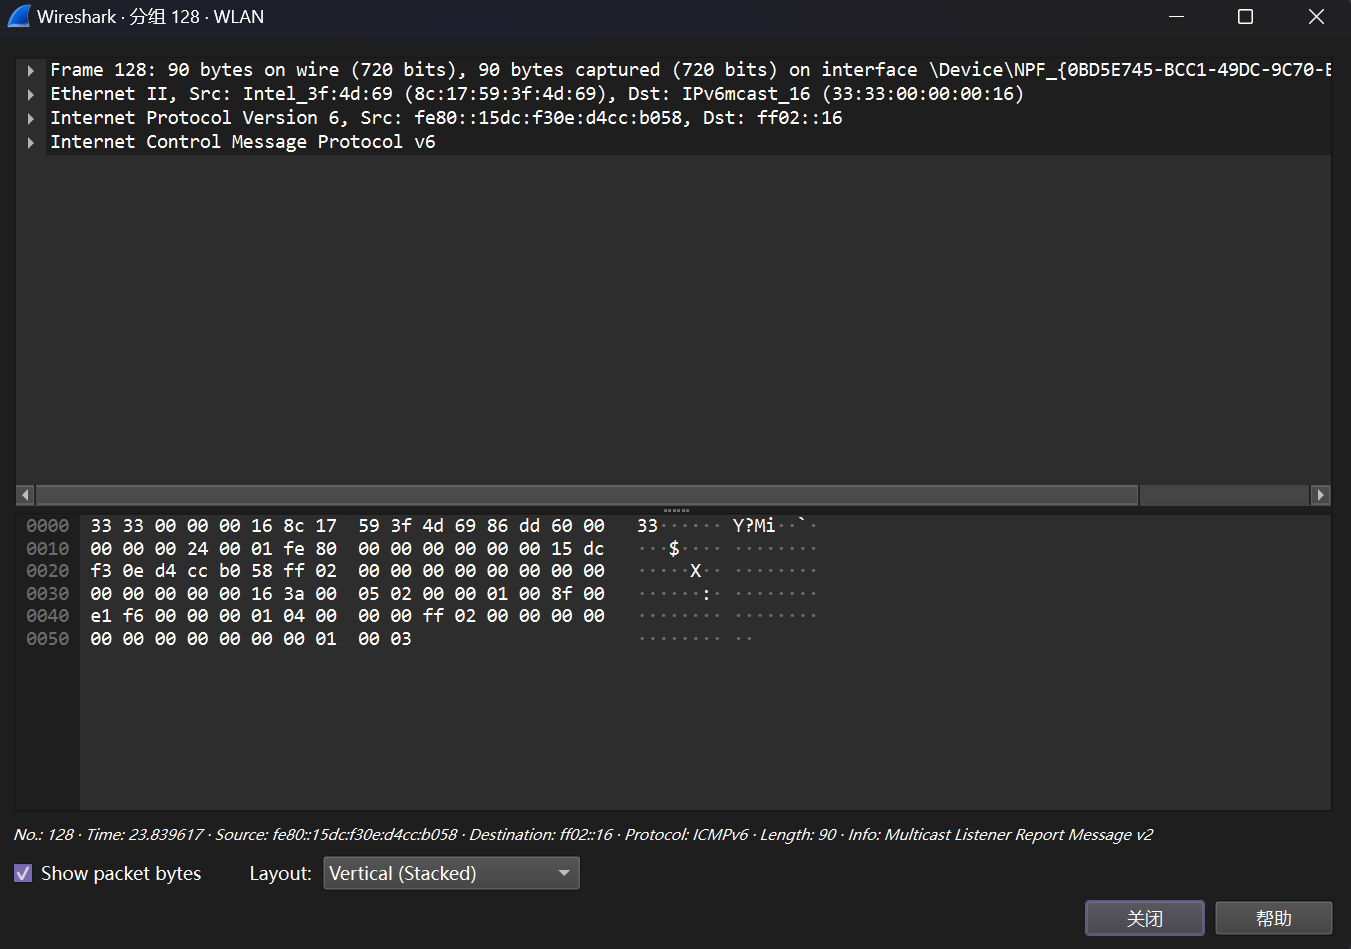
\includegraphics[width=11cm]{images/24. IPv6数据包结构.jpg}
			\caption{\texttt{IPv6}数据包结构}
			\label{fig:24}
		\end{figure}
		
		观察可知,IPv6数据包的构造与IPv4数据包存在明显差异。IPv6数据包的头部固定为40字节长,且其源地址和目的地址各占据16字节。与IPv4不同的是,IPv6数据包中不再包含校验和字段。此外,IPv6引入了Hop Limit字段,这一字段接替了IPv4中的TTL(Time to Live)字段的功能,用于控制数据包在网络中的传输跳数。
		
		\item Learn about tunnels, which wrap an IP packet within another IP header.
		
		隧道技术是一种网络通信方法,它允许将一个IP数据包嵌入到另一个IP数据包的头部之中。这种方法特别适用于不同IP版本之间的数据传输。具体来说,隧道技术能够实现IPv6数据包在IPv4网络中的传输,通过将IPv6数据包封装在IPv4数据包内来完成。反之,它也能够支持IPv4数据包在IPv6网络中的传输,即通过将IPv4数据包封装进IPv6数据包来实现。这种灵活性使得隧道技术成为IP版本转换和共存策略中的关键组成部分。
		
		\item Read about IP geolocation, It is the process of assigning a geographical location to an IP addressusing measurements or clues from its name administrative databases. Try a geolocation service.
		
		IP地理定位是一个技术过程,它将具体的地理位置与IP地址相关联。这一过程可以通过直接测量或通过查询IP地址的域名管理系统数据库来实现。为了进一步了解或应用IP地理定位,可以使用在线服务。例如,网站 \url{https://www.iplocation.net/} 提供了一项功能,允许用户通过输入IP地址来获取相关的地理信息。
		
		\item Learn about IPsec or IP security. It provides confidentiality and authentication for IP packets, and isoften used as part of VPNs.
		
		IPsec,即网际协议安全,是一种旨在增强IP数据包传输安全性的协议。它主要用于提供数据的保密性与发送者身份的验证,经常集成于虚拟私人网络(VPN)的架构中。IPsec通过在网络层对IP数据包实施加密和认证机制,保障信息在网络传输过程中的安全性,确保数据的机密性、完整性,并核实通信双方的身份,从而为网络通信提供了一道坚固的安全屏障。
		
	\end{enumerate}
	
	\section{实验结果总结}
	
	在本次实验中,我们通过Wireshark工具捕获了IP数据包,并对其进行了深入分析。具体步骤和发现如下:
	
	我们首先使用Wireshark捕获了网络中的IP数据包。接着,我们对IP数据包的结构进行了详细分析,并解答了与这些数据包相关的一系列问题。利用\texttt{tracert}命令,我们追踪了到达\url{www.baidu.com}的路由路径,并且绘制了相应的网络路径图。我们挑选了一个特定的IP数据包,并计算了其校验和(checksum)。
	
	在实验的最后阶段,我们对实验过程中遇到的问题进行了深入讨论。此外,我们还捕获并分析了IPv6数据包,以扩展我们对IP协议家族的理解。
	
	\section{附录}
	
	无
	
\end{document}